\extraPartText{\quotechapt{\personne{Alfvèn}[Hannes], un des pères de la physique des plasmas magnétisés.}{
  I have never thought that you could obtain the extremely clumpy, heterogeneous universe we have today, strongly affected by plasma processes, from the smooth, homogeneous one of the Big Bang, dominated by gravitation.\footnote{Traduction : Je n'ai jamais pensé que l'on pouvait obtenir l'univers hétérogène et très agité que nous connaissons aujourd'hui, fortement influencé par des processus plasmas, à partir de l'univers lisse et homogène du Big Bang, dominé par la gravitation. Citation extraite de \cite{peratt_dean_1988}.}}}

\part*{\linia
        \bigskip
        INTRODUCTION : La turbulence dans les plasmas astrophysiques
        \bigskip
        \linia}
   \addtocontents{toc}{\protect\vspace{2ex}\textbf{INTRODUCTION : Le vent solaire, un plasma turbulent non-collisionnel}\par}     
\setcounter{part}{-1}
\refstepcounter{part}\label{part_intro}
\renewcommand{\chaptername}{INTRODUCTION : Chapitre}
\renewcommand\Partie{INTRODUCTION : }
\setcounter{chapter}{0}


Quand on parle de turbulence, la première image qui résonne dans notre esprit est un écoulement semblant chaotique, des secousses dans un avion ou un enfant qui n'en fait qu'à sa tête. Les propriétés partagées par ces trois exemples sont l'agitation, l'apparent désordre, l'imprévisibilité. Mais ce n'est qu'apparence. Contrairement au pur chaos, ce comportement est statistiquement prévisible et peut montrer un semblant d'ordre. Dans ce chapitre, sont résumés des notions, notations et outils permettant de caractériser et de prédire le comportement d'un écoulement turbulent dans un cadre \cacro{HD}. 

\section{Définition et propriétés d'un écoulement turbulent}\label{sec-011}

 Supposons l'écoulement incompressible, c'est-à-dire un fluide de densité constante $\rho_0$. Ce fluide s'écoule à la vitesse $\boldsymbol{v}(t,\mathbf{x})$ dépendant du temps $t$ et de la position $\mathbf{x}$. L'hypothèse incompressible impose aussi une contrainte sur cette vitesse : l'annulation de sa divergence, c'est-à-dire, mathématiquement $\nabla \cdot \boldsymbol{v} = 0$ en notant $\nabla = \frac{\partial}{\partial \mathbf{x}}$ l'opérateur de dérivation spatiale.
 
 Un écoulement hydrodynamique incompressible est un système modélisé par les équations de Navier-Stockes incompressibles :
 \begin{eqnarray}
 \label{eq:navst_r} \nabla \cdot \boldsymbol{v} & =& 0 \\
 \label{eq:navst_v} \partial_t \boldsymbol{v} + \boldsymbol{v} \cdot \nabla \boldsymbol{v} &=& - \frac{1}{\rho_0} \nabla p + \nu \Delta \boldsymbol{v}.
 \end{eqnarray}
 Le premier terme de l'équation \eqref{eq:navst_v}, $\partial_t \boldsymbol{v}$, indique que cette équation est celle de l'évolution temporelle, $\partial_t = \frac{\partial}{\partial t}$ étant la dérivée partielle temporelle, de la vitesse de l'écoulement $\boldsymbol{v}$.
 Le deuxième terme, $\boldsymbol{v} \cdot \nabla \boldsymbol{v}$, implique un déplacement convectif du champ de vitesse à la vitesse de l'écoulement. Ce terme cristallise les non-linéarités du système. Dimensionnellement, on peut le schématiser par $C_{NL} = \frac{V^2}{L}$ avec $V$ la vitesse caractéristique de l'écoulement et $L$ sa largeur caractéristique.
 Le terme $- \frac{1}{\rho_0} \nabla p $ avec $p$ la pression du fluide dénote les forces de pressions impliquées dans l'écoulement.
 Le dernier terme, $\nu \Delta \boldsymbol{v}$, est un terme dissipatif, d'effort visqueux. Il dépend de $\nu$, la viscosité du fluide, et de $\Delta = \nabla^2$, l'opérateur Laplacien. Ce terme vient contrebalancer le terme convectif et, s'il domine, rend l'écoulement laminaire. On peut le schématiser tel que $C_{D} = \nu \frac{V}{L^2}$.
 
 Le rapport entre $C_{NL}$ et $C_D$ est le nombre de Reynolds $R_e = \frac{C_{NL}}{C_D} = \frac{VL}{\nu}$, un nombre sans dimension caractérisant le régime de l'écoulement, laminaire ($R_e$ faible) ou turbulent ($R_e \gg 1$). Ces régimes sont illustrés sur la \figref{fig:ecoulement}. Dans cette expérience, un jet d'eau (blanc) est injecté dans de l'eau stagnante (espace noir). À gauche, sa largeur caractéristique est imposée par le diamètre du tuyau d'injection, l'écoulement est alors dans un régime laminaire. Ensuite, la turbulence se développe (régime transitoire), il y a apparition de tourbillons (vortex) dans l'écoulement. Enfin, tout à droite, la turbulence est pleinement développée, les non-linéarités dominent et s'entretiennent.
 \begin{figure}[!ht]
  \centering
 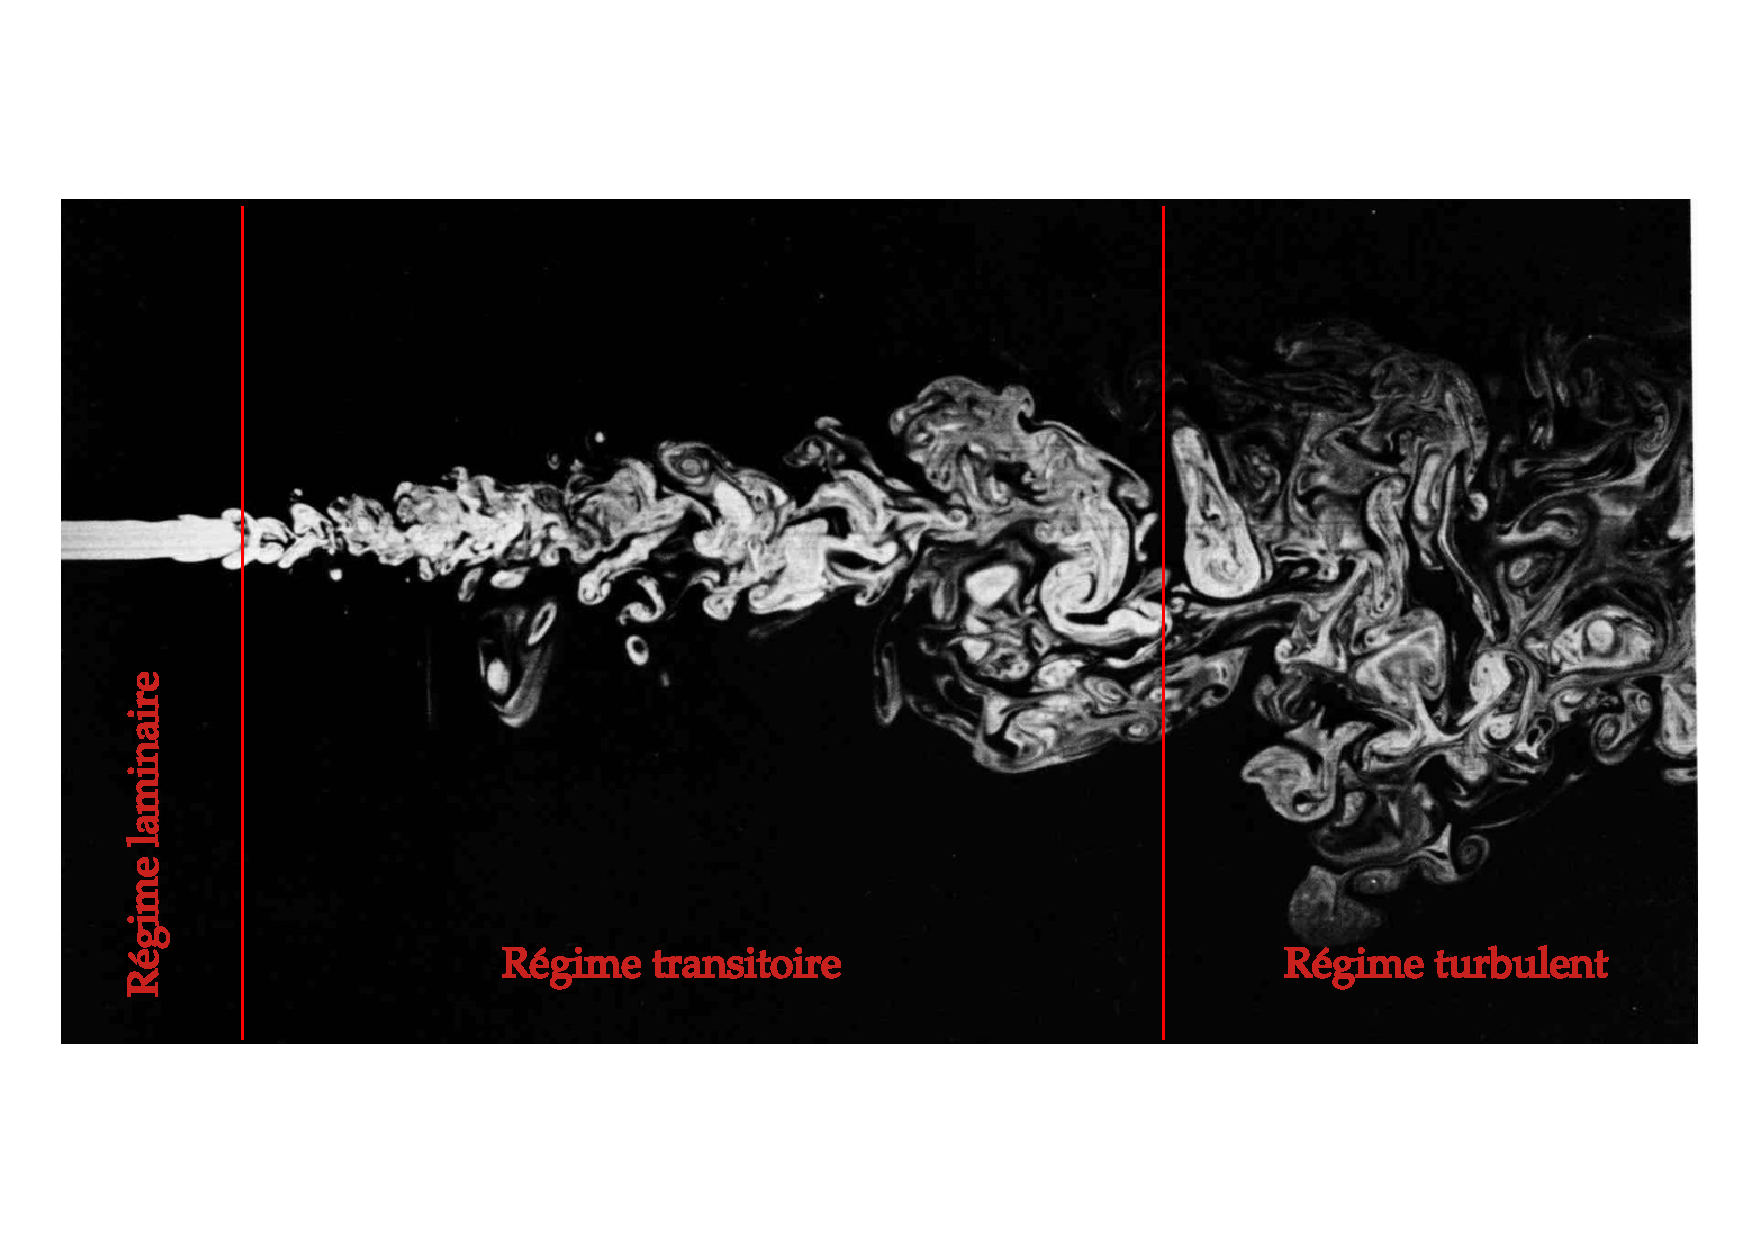
\includegraphics[width=\linewidth,trim=1cm 3cm 1cm 3cm, clip=true]{./Mainmatter/Part_0/images/turbul_Re}
 \caption{Injection d'un jet d'eau dans de l'eau observée par fluorescence laser et illustrant les différents régimes d'un écoulement : laminaire, transitoire et turbulent. [Crédits de l'image initiale : \cite{van_dyke_album_1982}.]}
 \label{fig:ecoulement}
 \end{figure}
 
 Dans le cadre hydrodynamique incompressible, l'écoulement n'est décrit que par les champs de vitesse et de pression, mais pour d'autres fluides, la description peut impliquer d'autres champs tels que le champ magnétique $\boldsymbol{B}$, le champ scalaire massique $\rho$, etc. On peut définir un nombre sans dimension similaire au nombre de Reynolds, rapport entre le terme non-linéaire convectif et le terme diffusif ou dissipatif impliqués dans l'évolution temporelle de ces champs. Dans le cas d'un champ magnétique, ce sera le nombre de Reynolds magnétique $R_m = \frac{VL}{\eta}$ avec $\eta$ la résistivité ou diffusivité magnétique. Pour des quantités thermodynamiques telles que la densité de masse ou la pression, on parlera plutôt de nombres de Péclet.
 
 Sur la \figref{fig:comp_turbul}, sont présentés des résultats d'une simulation turbulente \cacro{3D} qui sera introduite et utilisée dans la partie \ref{part_3}.
 \begin{figure}[!ht]
  \centering
 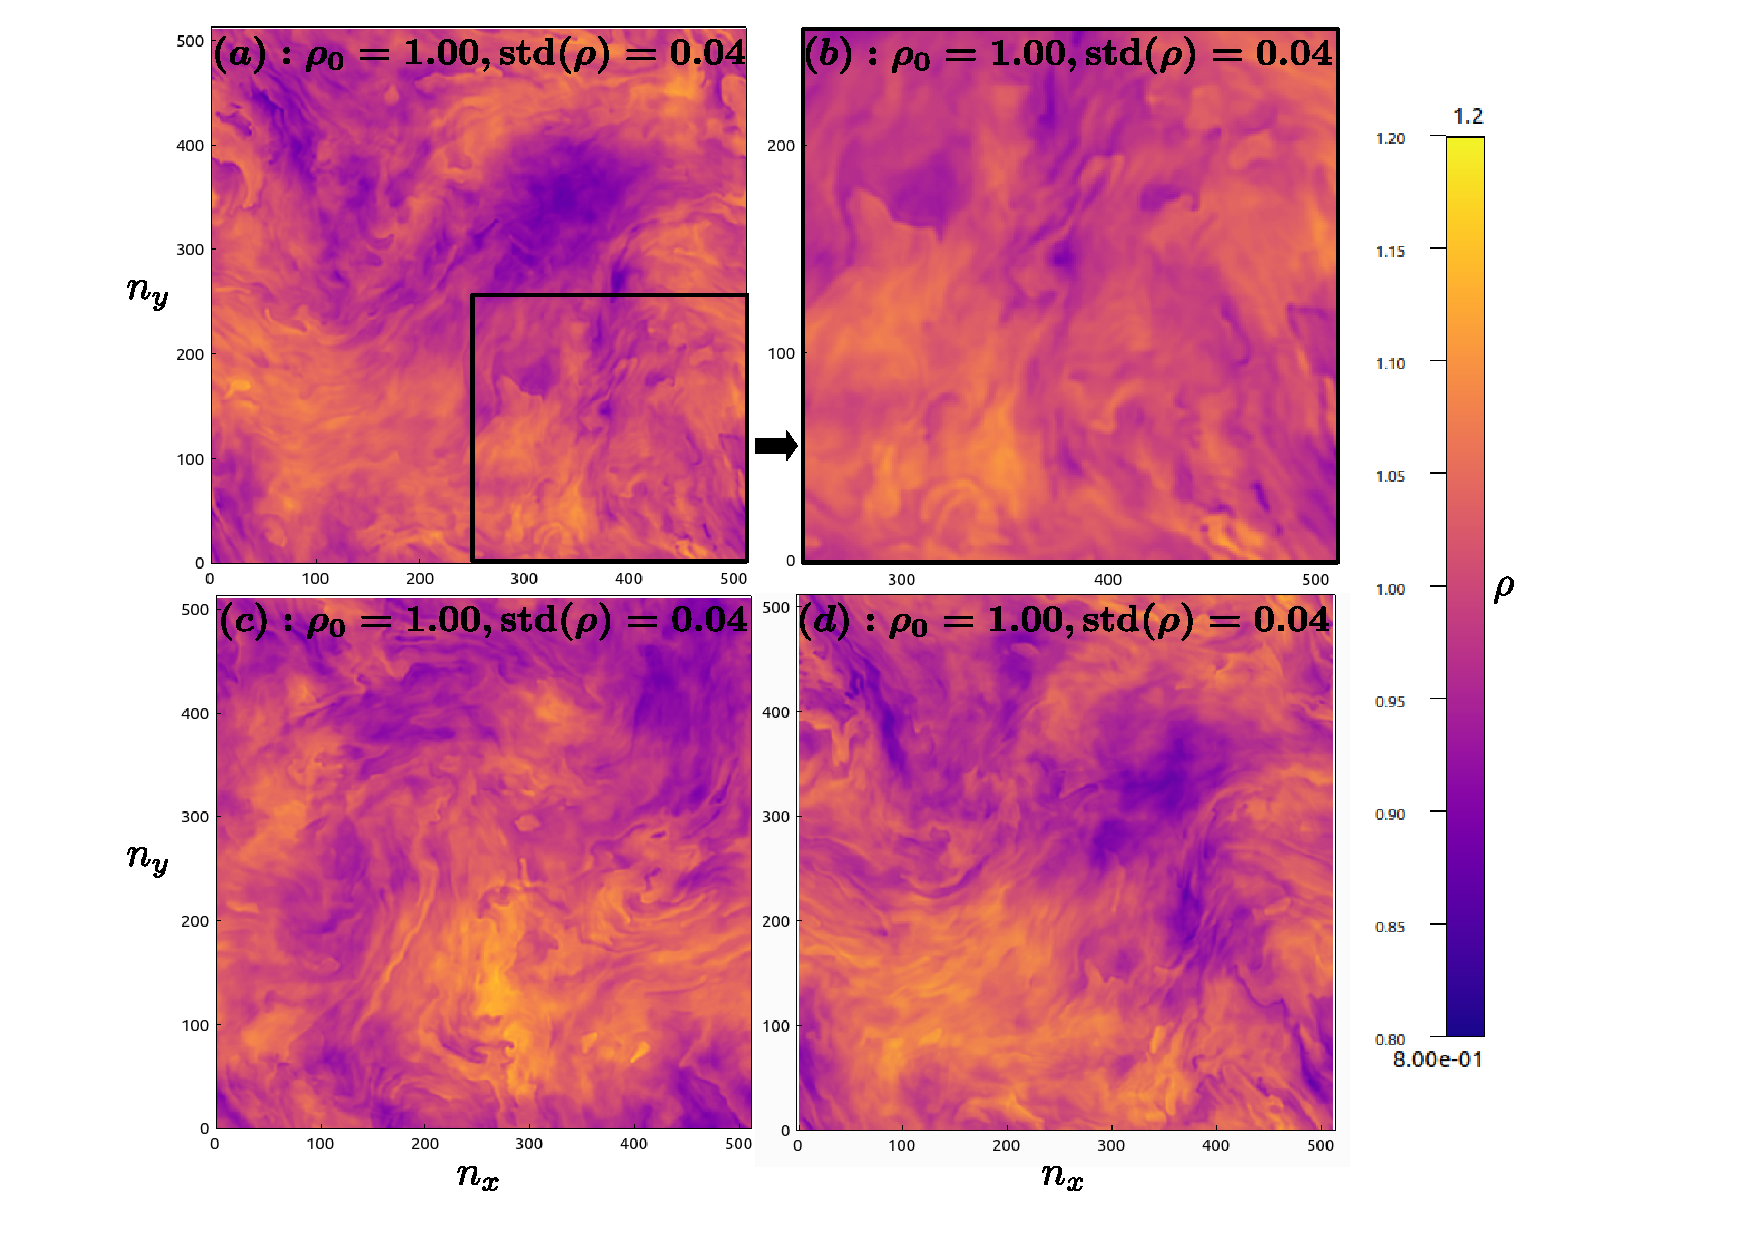
\includegraphics[width=0.8\linewidth,trim=2cm 0cm 4cm 0cm, clip=true]{./Mainmatter/Part_0/images/simu_panel_rho}
 \cprotect\caption{Résultats d'une simulation \cacro{3D} d'un plasma turbulent décrit par le modèle Hall-CGL. Le code de simulation sera introduit dans la partie \ref{part_3}. La quantité représentée est la densité $\rho$. Chaque image correspond à une coupe $x-y$ du cube de densité obtenu au temps $t$ (en unité de temps de la simulation). Les axes sont en position numérique (nombre de points dans chaque direction, comptés à partir d'une position $(0,0,0)$). (a) : $n_z=323$, $t=410$. (b) : zoom de (a). (c) : $n_z=638$, $t=410$. (d) : $n_z=323$, $t=408$. Pour chaque image, la moyenne spatiale, $\rho_0$, est de $\num{1.00}$ et l'écart-type, $\text{std}(\rho)$, de $\num{0.04}$.}
 \label{fig:comp_turbul}
 \end{figure}
 L'image (a) correspond à une coupe du cube de densité $\rho$ telle que $n_z=323$ obtenue au temps $t=410$. Si on la compare à l'image (c) (autre coupe du même cube telle que $n_z=638$), on remarque une certaine invariance spatiale statistique qui illustre la propriété d'homogénéité dite statistique d'un fluide turbulent. Si par contre, on la compare à l'image (d) (coupe $n_z=323$ obtenue à la date $t=408$), on retrouve similairement une certaine invariance temporelle qui vient illustrer la propriété de stationnarité statistique du fluide. Enfin, en comparant avec l'image (b) (zoom de l'image (a)), on observe ce qui semble être une loi d'échelle.
 
 Un écoulement ou un fluide turbulent serait donc caractérisé par
 \begin{itemize}
 \item une dominance des non-linéarités sur les contributions diffusives (grands nombres de Reynolds et de Péclet),
 \item des propriétés d'invariance (homogénéité, stationnarité) au sens statistique,
 \item une loi d'échelle.
 \end{itemize}
 Dans la section \ref{sec-012}, on va définir les notations et appellations liées aux notions mathématiques statistiques et dans la section \ref{sec-013}, on abordera un peu plus en détail la description de la turbulence à travers les échelles.
 
\section{Description statistique et notations pour l'étude d'un système turbulent}\label{sec-012}

Afin de garder la description du travail présenté dans ce mémoire accessible à tous, nous ne nous perdrons pas dans des définitions mathématiques complexes et exhaustives des notions, mais resterons sur des définitions exemplifiées et plus appliquées. 

Dans l'ensemble de ce mémoire, on se placera dans un cadre \cacro{3D}. Sauf quantités indéfinies, les grandeurs vectorielles seront notées en gras. Le système de représentation spatial sera génériquement cartésien $\mathbf{x} = (x,y,z)$, sauf mention contraire.

Soit une quantité indéfinie $X$ (densité, vitesse, pression, champ magnétique, etc.) caractérisant un fluide. La distribution de valeurs possibles pour $X$, ou distribution de probabilité de $X$, notée $\mathcal{P}_X$, peut être obtenue en considérant différents points de vue :
\begin{itemize}
    \item PV1 : décrire le fluide comme un ensemble souvent discret, par exemple de $N$ particules (atomes, molécules, etc.) associées individuellement à une valeur de la quantité $X$, notée $X_n$ avec $n \in [1;N]$,
    \item PV2 : regarder l'espace occupé par le fluide : un volume continu $V$ ou un nombre de points d'emplacement $\mathbf{x}$. La quantité $X$ sera alors évaluée en chacun d'eux et notée $X(\mathbf{x})$, 
    \item PV3 : ne considérer qu'une particule ou qu'un point, regarder les valeurs de $X$ au fil du temps sur une période $T$, et les noter $X(t)$. 
\end{itemize}
Ces différents points de vue ne sont pas forcément équivalents. Par exemple, si l'on regarde plusieurs types de particules et que les valeurs de $X$ dépendent de leur nature, ne regarder qu'une particule au fil du temps ne sera pas représentatif du système. Par la suite, on utilisera les représentations PV2 et PV3.  

Pour caractériser la distribution de probabilité de $X$, on peut utiliser divers outils statistiques. L'un d'eux est la moyenne (moment d'ordre 0), une opération linéaire que l'on va noter $\left< X \right>$ et qui est définie en fonction des points de vue :
\begin{itemize}
    \item PV1 : $\left<X\right>_{N} = \frac{1}{N} \sum_{n=1}^N X_n$, est la moyenne d'ensemble définie de manière discrète.
    \item PV2 : $\left<X\right>_{V} = \frac{1}{V} \int_V X(\mathbf{x}) \mathcal{P}_X d\mathbf{x}$, est la définition continue de la moyenne spatiale. $\left<X\right>_V$ est indépendante de la position locale $\mathbf{x}$. Dans le cas discret, en considérant un échantillonnage spatial, c'est-à-dire $N_V$ points dans le volume $V$, et en notant $X_p$ la valeur de $X$ au point $p$, $\left<X\right>_{V} = \frac{1}{N_V} \sum_{p=1}^{N_V} X_p$. 
    \item PV3 : $\left<X\right>_{T} = \frac{1}{T} \int_0^T X(t) \mathcal{P}_X dt$, est la définition continue de la moyenne temporelle. $\left<X\right>_T$ est indépendante de l'instant $t$. Une moyenne discrète peut aussi être définie en considérant un échantillonnage temporel.
\end{itemize}
Si $\left<X\right>_{N} = \left<X\right>_{V} = \left<X\right>_{T}$ est vérifiée, on peut supposer une équivalence statistique des différents points de vue. Le système sera alors ergodique. 

On peut définir plus rigoureusement les propriétés d'homogénéité et de stationnarité statistiques à l'aide de $\mathcal{P}_X$ : 
\begin{itemize}
    \item \textbf{\emph{homogénéité statistique}} : soient deux échantillons représentatifs du système et définis relativement à deux positions indépendantes l'une de l'autre $\mathbf{x}$ et $\mathbf{x'}$ alors  $\mathcal{P}_X(\mathbf{x}) = \mathcal{P}_X(\mathbf{x'}) = \mathcal{P}_X$, ce qui implique pour la moyenne $\left<X(\mathbf{x})\right> = \left<X(\mathbf{x'})\right> = \left<X\right>$,
    \item \textbf{\emph{stationnarité statistique}} : soient deux échantillons représentatifs du système et définis relativement à deux instants indépendants l'un de l'autre $t$ et $t'$ alors $\mathcal{P}_X(t) = \mathcal{P}_X(t') = \mathcal{P}_X$, ce qui implique pour la moyenne $\left<X(t)\right> = \left<X(t')\right> = \left<X\right>$.
\end{itemize}
Attention, cela ne signifie pas que localement, entre deux instants $t$ ou deux positions $\mathbf{x}$, $X$ sera constant. En pratique, dans des données d'observations ou de simulations, des échantillons dans lesquels ces hypothèses seraient parfaitement valides sont difficiles à obtenir. Des compromis devront donc être établis. 

Similairement aux définitions des propriétés d'homogénéité et de stationnarité statistiques, pour étudier un fluide turbulent, on doit relier le comportement statistique de deux échantillons ou plus, c'est-à-dire que l'on doit s'intéresser aux fluctuations, incréments de quantités et corrélations entre au moins deux échantillons. Ce lien peut s'exprimer en fonction de la distance temporelle ou spatiale entre ces échantillons, généralement appelée <<échelle>>. En 1941, Kolmogorov pose les bases d'une théorie permettant d'obtenir une telle relation : la théorie des lois exactes [\cite{frisch_turbulence_1995,kolmogorov_dissipation_1991,kolmogorov_local_1991}]. Cette théorie repose sur les hypothèses que nous avons illustrées dans la section \ref{sec-011} (dominance des effets non-linéaires, homogénéité et stationnarité statistiques) ainsi que sur une hypothèse plus spécifique de séparation d'échelle qui sera expliquée dans la section \ref{sec-013}.

Le travail décrit dans ce mémoire est basé sur cette théorie et implique les notations suivantes. On considèrera deux échantillons définis relativement à deux positions\footnote{Il est possible de corréler plus de deux points. Tout lecteur intéressé pourra se référer à [\cite{cho_simulations_2009}].}\footnote{Historiquement, les calculs sont effectués dans le cadre PV2. Il serait a priori possible de les transposer dans les cadres PV1 ou PV3, mais ce n'est pas l'objet de cette thèse.} indépendantes l'une de l'autre, $\mathbf{x}$ et $\mathbf{x'}$. La quantité indéfinie $X$ évaluée en $\mathbf{x'}$ sera notée $X'$ et celle évaluée en $\mathbf{x}$, $X$. L'échelle, notée $\boldsymbol{\ell}$, sera définie comme l'incrément de position : 
\begin{equation}
    \boldsymbol{\ell} = \delta \mathbf{x} = \mathbf{x'} - \mathbf{x} ,
\end{equation}
avec $\delta$ dénotant le caractère incrémental. Similairement l'incrément de la quantité indéfinie $X$ s'écrira : 
\begin{equation}
    \delta X = X' - X = X(\mathbf{x'}) - X(\mathbf{x})  .
\end{equation}

Le lien étudié entre les deux échantillons sera une fonction de corrélation spatiale entre deux quantités $X$ et $Y$ (ici indéfinies) qui s'obtient en considérant une quantité au point $\mathbf{x}$ et l'autre au point $\mathbf{x'}$, en les multipliant puis en moyennant. Afin de conserver une symétrie du rôle de $\mathbf{x}$ et $\mathbf{x'}$, on définira la fonction de corrélation telle que 
\begin{equation}
    \label{eq:def_correlation} \mathcal{R}_{XY} = \frac{1}{2} \left<X \cdot Y' + X' \cdot Y\right>,
\end{equation}
en notant $\cdot$ l'opération générique multiplicative. Entre deux vecteurs, cette opération pourrait être considérée comme un produit scalaire ou remplacée par un produit vectoriel noté $\times$. La fonction d'auto-corrélation est obtenue en considérant $X=Y$, c.-à-d. $\mathcal{R}_{XX} = \left<X \cdot X'\right>$. 
La moyenne $\left<\right>$ impliquée dans ces fonctions est la moyenne spatiale. $\mathcal{R}_{XY}$ sera donc indépendante de $\mathbf{x}$ et $\mathbf{x'}$ et ne dépendra que de $\boldsymbol{\ell}$ et a priori de $t$ si les quantités dépendent du temps. 

Par indépendance entre le temps et la position, la moyenne spatiale commute avec la dérivée temporelle : 
\begin{equation}
  \label{eq:prop_t}  \partial_t \left<X\right> = \left<\partial_t X\right> .
\end{equation}
On note  $\nabla_{\boldsymbol{\ell}} = \frac{\partial}{\partial \boldsymbol{\ell}}$ l'opérateur de dérivation spatiale dans l'espace global des échelles, $\nabla$ et $\nabla'$ les opérateurs de dérivation locaux respectivement en $\mathbf{x}$ et $\mathbf{x'}$. L'indépendance entre $\mathbf{x}$ et $\mathbf{x'}$, implique que :
\begin{equation}
  \label{eq:prop_x}    \nabla X' = 0,  \qquad \nabla' X = 0.
\end{equation}
Grâce à l'hypothèse d'homogénéité statistique, ces opérateurs dérivatifs vérifient\footnote{
Soient $A$, $B$ et $C$ des quantités indéfinies telles que $A(\boldsymbol{\ell}) = \left<B \cdot C'\right> = \left<B(\mathbf{x}) \cdot C(\mathbf{x'})\right>$  avec $\cdot$ une opération multiplicative quelconque et $\mathbf{x'} = \mathbf{x} + \boldsymbol{\ell}$. Alors, l'élément différentiel $d \boldsymbol{\ell} $ est égal à $d \mathbf{x'} - d \mathbf{x}$. 

À $\mathbf{x}$ fixé, $ d \boldsymbol{\ell} = d \mathbf{x'}$, alors
$\nabla_{\boldsymbol{\ell}} A(\boldsymbol{\ell}) = \left<\partial_{\boldsymbol{\ell}} (B \cdot  C')\right> = \left<\partial_{\mathbf{x'}} (B \cdot  C') \right> = \left<\nabla' (B \cdot  C')\right> $. D'où la relation entre les opérateurs :  $\nabla_{\boldsymbol{\ell}} \left<\right> = \left<\nabla'\right>$. Similairement, à $\mathbf{x'}$ fixé, $ d \boldsymbol{\ell} = - d \mathbf{x}$, d'où $\nabla_{\boldsymbol{\ell}} \left<\right> = - \left<\nabla\right>$.
}
\begin{equation}
   \label{eq:prop_l}   \nabla_{\boldsymbol{\ell}}\left<\right> = \left<\nabla' \right> = - \left<\nabla \right> .
\end{equation}

En turbulence, on utilise aussi communément la transformée de Fourier. Cette méthode permet de travailler dans un espace où la position est repérée par $\boldsymbol{k} \propto 1/\mathbf{x}$, et où toute quantité se retrouve décomposée en une série de \og modes \fg{} que l'on appelle un spectre. Dans le cas continu \cacro{3D}, on définit la transformée de Fourier de la quantité $X$ par 
\begin{equation}
    \tilde{X}(\boldsymbol{k}) = \frac{1}{(2\pi)^3} \iiint X(\mathbf{x}) e^{-i\boldsymbol{k} \cdot \mathbf{x}} d\mathbf{x}
\end{equation}
et la transformée inverse par 
\begin{equation}
    X(\mathbf{x}) = \iiint \tilde{X}(\boldsymbol{k}) e^{i\boldsymbol{k} \cdot \mathbf{x}} d\boldsymbol{k}.
\end{equation} 
On remarque qu'en termes de dimensions, si l'on note $[X]$ l'unité de $X$ et $L$ l'unité de longueur, $\tilde{X} \sim [X] L^3$.

Dans le cas continu \cacro{1D}, on aura similairement : 
\begin{equation}
    \tilde{X}(k) = \frac{1}{2\pi} \int X(x) e^{-ikx} dx , \qquad 
    X(x) = \int \tilde{X}(k) e^{ikx} dk
\end{equation} 
et en termes de dimensions, $\tilde{X} \sim [X] L$.

Ces notations et hypothèses seront utilisées tout au long de ce mémoire. Pour se familiariser avec leur utilisation, une application de la théorie de Kolmogorov à un écoulement hydrodynamique incompressible décrit par les équations de Navier-Stockes \eqref{eq:navst_r} et \eqref{eq:navst_v} est donnée dans la section \ref{sec-013}. Cette application va nous servir à introduire la notion de loi d'échelle et l'hypothèse de séparation d'échelle.



 \section{Théorie de Kolmogorov et loi d'échelle}\label{sec-013}
 
 La démonstration de Kolmogorov de 1941 [version traduite :  \cite{kolmogorov_dissipation_1991,kolmogorov_local_1991}] a été réécrite à de multiples reprises sous différentes formes. D'autres versions sont données par \cite{monin_statistical_1975}, \cite{frisch_turbulence_1995}, \cite{antonia_analogy_1997}, et \cite{galtier_physique_2021}. 
 
Pour faciliter les étapes de calcul, on va réécrire l'équation de Navier-Stockes \eqref{eq:navst_v} grâce à l'hypothèse incompressible \eqref{eq:navst_r} et y ajouter un terme de forçage $\boldsymbol{f_c}$ : 
\begin{equation}
  \label{eq:navst_v2}  \partial_t \boldsymbol{v} = - \nabla \cdot (\boldsymbol{v} \boldsymbol{v}) -  \frac{1}{\rho_0} \nabla p + \nu \Delta \boldsymbol{v} + \boldsymbol{f_c} 
.\end{equation}

La démonstration se base sur la recherche d'une équation d'évolution temporelle pour la fonction d'auto-corrélation $\mathcal{R}_{\boldsymbol{v}\boldsymbol{v}} = \left<\boldsymbol{v} \cdot \boldsymbol{v'}\right>$. Pour l'obtenir, on dérive temporellement $\mathcal{R}_{\boldsymbol{v}\boldsymbol{v}}$ grâce à la propriété \eqref{eq:prop_t} (étape \eqref{eq:step_1}), on injecte l'équation de Navier-Stockes \eqref{eq:navst_v2} (étape \eqref{eq:step_2}) puis on applique les propriétés \eqref{eq:prop_x} et \eqref{eq:prop_l} pour extraire les opérateurs dérivatifs spatiaux de la moyenne spatiale (étape \eqref{eq:step_3}) : 
\begin{eqnarray}
    \partial_t \mathcal{R}_{\boldsymbol{v}\boldsymbol{v}} &=& \left<\boldsymbol{v} \cdot \partial_t \boldsymbol{v'} + \boldsymbol{v'} \cdot \partial_t \boldsymbol{v}\right> \label{eq:step_1} \\ 
    &=& - \left< \nabla' \cdot (\boldsymbol{v'} \boldsymbol{v'}) \cdot \boldsymbol{v}   +  \nabla \cdot (\boldsymbol{v} \boldsymbol{v})\cdot\boldsymbol{v'} \right> - \frac{1}{\rho_0} \left<\boldsymbol{v} \cdot \nabla' P' + \boldsymbol{v'} \cdot \nabla P\right>  \nonumber \\
    && + \nu \left<\boldsymbol{v} \cdot \Delta' \boldsymbol{v'} + \boldsymbol{v'} \cdot \Delta \boldsymbol{v}\right> + \left<\boldsymbol{v} \cdot \boldsymbol{f'_c} + \boldsymbol{v'} \cdot \boldsymbol{f_c}\right> \label{eq:step_2} \\  
    &=& \nabla_{\boldsymbol{\ell}} \cdot \left< - \boldsymbol{v} \cdot \boldsymbol{v'} \boldsymbol{v'} + \boldsymbol{v'} \cdot \boldsymbol{v} \boldsymbol{v}\right>  + \frac{1}{\rho_0} \nabla_{\boldsymbol{\ell}} \cdot \left< - P' \boldsymbol{v} + P \boldsymbol{v'}\right> \nonumber \\
    && + 2 \nu \Delta_{\boldsymbol{\ell}} \left<\boldsymbol{v} \cdot \boldsymbol{v'} \right>  + \left<\boldsymbol{v} \cdot \boldsymbol{f'_c} + \boldsymbol{v'} \cdot \boldsymbol{f_c}\right>  \label{eq:step_3}  
.\end{eqnarray}
Avec l'hypothèse incompressible et celle d'homogénéité statistique (propriétés \eqref{eq:prop_x} et \eqref{eq:prop_l}), 
\begin{eqnarray}
    \nabla_{\boldsymbol{\ell}} \cdot \left< - P' \boldsymbol{v} + P \boldsymbol{v'}\right> &=& 0, \\
    \nabla_{\boldsymbol{\ell}} \cdot \left< - \boldsymbol{v} \cdot \boldsymbol{v'} \boldsymbol{v'} + \boldsymbol{v'} \cdot \boldsymbol{v} \boldsymbol{v}\right> &=& \frac{1}{2} \nabla_{\boldsymbol{\ell}} \cdot \left< \delta \boldsymbol{v} \cdot \delta \boldsymbol{v} \delta \boldsymbol{v} \right>, \\
    \left<\boldsymbol{v} \cdot \boldsymbol{f'_c} + \boldsymbol{v'} \cdot \boldsymbol{f_c}\right> &=& \left<\boldsymbol{v} \cdot \left(\boldsymbol{f_c}\left(\mathbf{x}+\boldsymbol{\ell}\right) +  \boldsymbol{f_c}\left(\mathbf{x}-\boldsymbol{\ell}\right)\right)\right>
.\end{eqnarray}

D'où l'équation dite \cacro{KHM}: 
\begin{equation}
    - \frac{\rho_0}{2} \partial_t \mathcal{R}_{\boldsymbol{v}\boldsymbol{v}} + \nu \rho_0 \Delta_{\boldsymbol{\ell}} \mathcal{R}_{\boldsymbol{v}\boldsymbol{v}} + \frac{\rho_0}{2} \left<\boldsymbol{v} \cdot \left(\boldsymbol{f_c}\left(\mathbf{x}+\boldsymbol{\ell}\right) +  \boldsymbol{f_c}\left(\mathbf{x}-\boldsymbol{\ell}\right)\right)\right> = - \frac{\rho_0}{4} \nabla_{\boldsymbol{\ell}} \cdot \left<\delta \boldsymbol{v} \cdot \delta \boldsymbol{v} \delta \boldsymbol{v}\right> \label{eq:KHM_HD}  
.\end{equation} 

Schématiquement, on va la noter : 
\begin{equation}
    \label{eq:bal_KHM} -\partial_t \mathcal{R} + \varepsilon_{NL} + \varepsilon_{F} + \varepsilon_{D} = 0 .
\end{equation} 
\begin{itemize}
    \item $\mathcal{R} = \frac{\rho_0}{2} \mathcal{R}_{\boldsymbol{v}\boldsymbol{v}}$, la fonction de corrélation de densité d'énergie totale (ici cinétique). En $\boldsymbol{\ell} = 0$, elle est égale à la densité d'énergie totale moyenne $\left<\frac{\boldsymbol{v}^2}{2}\right>$ du système.
    \item $\varepsilon_{NL} = \frac{1}{4} \rho_0 \nabla_{\boldsymbol{\ell}} \cdot \left<\delta \boldsymbol{v} \cdot \delta \boldsymbol{v} \delta \boldsymbol{v}\right>$, le taux de cascade ou de transfert non-linéaire de l'énergie incrémentale $\frac{1}{4} \rho_0 \left<\delta \boldsymbol{v}^2\right>$ à travers les échelles, il s'annule en $\boldsymbol{\ell} = 0$.
    \item $\varepsilon_{F} = \frac{1}{2} \rho_0 \left<\boldsymbol{v} \cdot \left(\boldsymbol{f_c}\left(\mathbf{x}+\boldsymbol{\ell}\right) +  \boldsymbol{f_c}\left(\mathbf{x}-\boldsymbol{\ell}\right)\right)\right>$, le taux de forçage dépendant des échelles. En $\boldsymbol{\ell} = 0$, il est égal à la densité d'énergie moyenne injectée $\rho_0 \left<\boldsymbol{v} \cdot  \boldsymbol{f_c}\right>$ dans le système par le forçage.
    \item $\varepsilon_{D} = \rho_0 \nu \Delta_{\boldsymbol{\ell}} \mathcal{R}_{\boldsymbol{v}\boldsymbol{v}}$, le taux de dissipation dépendant des échelles. En $\boldsymbol{\ell} = 0$, il est égal à la densité d'énergie moyenne dissipée par viscosité $\rho_0 \nu \left<\Delta \boldsymbol{v}^2\right>$.
\end{itemize}

On remarque qu'en $\boldsymbol{\ell} = 0$, \eqref{eq:KHM_HD} devient l'équation d'énergie totale moyenne que l'on peut noter : 
\begin{equation}
     \label{eq:bal_KHM0} -  \partial_t \mathcal{R}(\boldsymbol{\ell} =0)  + \varepsilon_{D}(\boldsymbol{\ell} =0) +  \varepsilon_{F}(\boldsymbol{\ell} =0) = 0  
.\end{equation} 

L'hypothèse de stationnarité statistique vient annuler toute dérivée temporelle de quantités moyennées. Par conséquent, les équations \eqref{eq:bal_KHM} et \eqref{eq:bal_KHM0} deviennent :  
\begin{eqnarray}
    \label{eq:bal_eps}\varepsilon_{NL} + \varepsilon_{F} + \varepsilon_{D} &=& 0 ,\\
    \label{eq:bal_eps0} \varepsilon_{D}(\boldsymbol{\ell} =0) +  \varepsilon_{F}(\boldsymbol{\ell} =0) &=& 0
.\end{eqnarray}


Les démonstrations existantes divergent dans le traitement des taux $\varepsilon_{F}$ et $\varepsilon_{D}$ de l'équation \eqref{eq:bal_eps} car elles ne prennent pas forcément en compte $\varepsilon_{F}$. Mais, toutes utilisent une propriété fondamentale de la turbulence, la loi <<zéroième>>. Cette loi indique que, pour un nombre de Reynolds grand, lorsque $\nu$ tend vers 0, la densité d'énergie dissipée moyenne $\rho_0 \nu  \left<\Delta\boldsymbol{v}^2\right>$, qui correspond à  $\varepsilon_D$ évalué en $\boldsymbol{\ell} =0$, devient indépendante de $\nu$ et ne s'annule pas. Cette singularité est aussi appelée anomalie dissipative. Elle indique la présence d'une dissipation dans la limite $R_e \gg 1$. On va noter $-\varepsilon$ cette valeur particulière de  $\varepsilon_D$. On peut alors résumer cette loi comme suit : 
\begin{equation}
 \label{eq:zero}  \varepsilon_D  \xrightarrow[\nu \rightarrow 0]{} \left\{
    \begin{aligned}
    & 0 & \textrm{si $\boldsymbol{\ell} \neq 0$ } \\
& - \varepsilon &  \textrm{si $\boldsymbol{\ell} =0$ } 
\end{aligned}
\right. .
\end{equation}

Si l'on prend en compte le terme de forçage, il sera supposé actif aux grandes échelles, notées $\boldsymbol{\ell_F} $. Aux échelles $\boldsymbol{\ell} \ll \boldsymbol{\ell_F}$, on obtient\footnote{Une démonstration de cette approximation est donnée dans l'Annexe \ref{an:forc} pour un forçage de type distribution de Dirac dans l'espace de Fourier.} $\varepsilon_{F} = \varepsilon_{F}(\boldsymbol{\ell} =0)$.  Avec la relation \eqref{eq:bal_eps0} et la loi zéroième \eqref{eq:zero}, on obtient alors $\varepsilon_{F}(\boldsymbol{\ell} \ll \boldsymbol{\ell_F}) = \varepsilon$. Enfin, en se plaçant à des échelles différentes de $\boldsymbol{\ell} =0$, telles que $\varepsilon_{D}=0$, on obtient de \eqref{eq:bal_eps}, la loi exacte \cacro{K41} : 
 \begin{equation}
  \label{eq:led_kolm} \frac{\varepsilon}{\rho_0} = - \frac{1}{4} \nabla_{\boldsymbol{\ell}} \cdot \left<\delta \boldsymbol{v} \cdot \delta \boldsymbol{v} \delta \boldsymbol{v}\right>
 \end{equation}
 qui s'écrit schématiquement $\varepsilon=-\varepsilon_{NL}$. Dans ce mémoire, nous déterminerons et analyserons $\varepsilon_{NL}$ pour différents modèles. Si l'on ne prend pas en compte le terme de forçage, on peut construire la différence entre \eqref{eq:bal_KHM} et \eqref{eq:bal_KHM0} et, dans la limite des grands nombres de Reynolds et avec l'hypothèse de stationnarité statistique, on peut retrouver \eqref{eq:led_kolm} [\cite{antonia_analogy_1997}]. 
 
 Cette loi est valable dans une gamme d'échelle dite inertielle où le comportement du fluide est supposé complètement non-linéaire ($R_e \gg 1$ et $\nu \rightarrow 0$) et peu impacté par tout phénomène d'injection d'énergie. La cascade d'énergie s'y effectue donc à un taux $\varepsilon$ constant. L'ensemble des dernières hypothèses est résumé sous le nom \textbf{\emph{\og hypothèse de séparation d'échelle \fg{} : 
 il existe une gamme d'échelle dite inertielle où l'énergie cascade conservativement (pas de dissipation, $\nu \rightarrow 0$ et $\boldsymbol{\ell} \neq 0$, ni de forçage, $\boldsymbol{\ell} \ll \boldsymbol{\ell_F}$) à un taux $\varepsilon$ constant.}} 
 
 Une autre hypothèse, communément appliquée en hydrodynamique, a été prise en compte par Kolmogorov, celle d'isotropie statistique. Elle permet d'obtenir une forme intégrée de la loi exacte. L'isotropie statistique implique une invariance angulaire sphérique. $\varepsilon(\boldsymbol{\ell})$ ne dépendra alors que de $\ell = |\boldsymbol{\ell}|$. On peut alors intégrer sur une boule de rayon $\ell$ la loi \eqref{eq:led_kolm} sachant que, dans la zone inertielle, $\varepsilon$ est constant. Ainsi, en notant $v_{\ell} = \boldsymbol{v} \cdot \boldsymbol{\ell}$, on a : 
 \begin{equation}
   \label{eq:kolmogorov}  - \frac{4}{3} \frac{\varepsilon}{\rho_0} \ell = \left<|\delta \boldsymbol{v}|^2 \delta v_{\ell}\right>.
 \end{equation}
 
 Phénoménologiquement, par analyse dimensionnelle, la loi exacte \eqref{eq:kolmogorov} s'écrit $(\delta v)^3 \sim \ell$ d'où $E(\ell) \sim (\delta v)^2 \sim \ell^{2/3}$. En passant dans l'espace de Fourier, sachant que l'on se place dans un cas \cacro{1D}, on peut remplacer $\ell$ par $1/k$ et $E(\ell)$ par $k E(k)$. On obtient alors le spectre énergétique :
 \begin{equation}
     E(k) \sim k^{-5/3}.
 \end{equation} 
 D'où, en représentation logarithmique, $\log E(k) = -5/3 \log k + C $ avec $C$ une constante. Ainsi, la théorie de Kolmogorov nous permet de prédire, dans le cas isotrope, un spectre d'énergie cinétique, $E(k)$ de pente $-5/3$ en représentation logarithmique. Malgré son caractère phénoménologique, cette prédiction est très bien retrouvée sur plusieurs ordres de grandeurs, par exemple dans le cadre expérimental (voir  \figref{fig:spec_kolmo}). 
 \begin{figure}[]
  \centering
 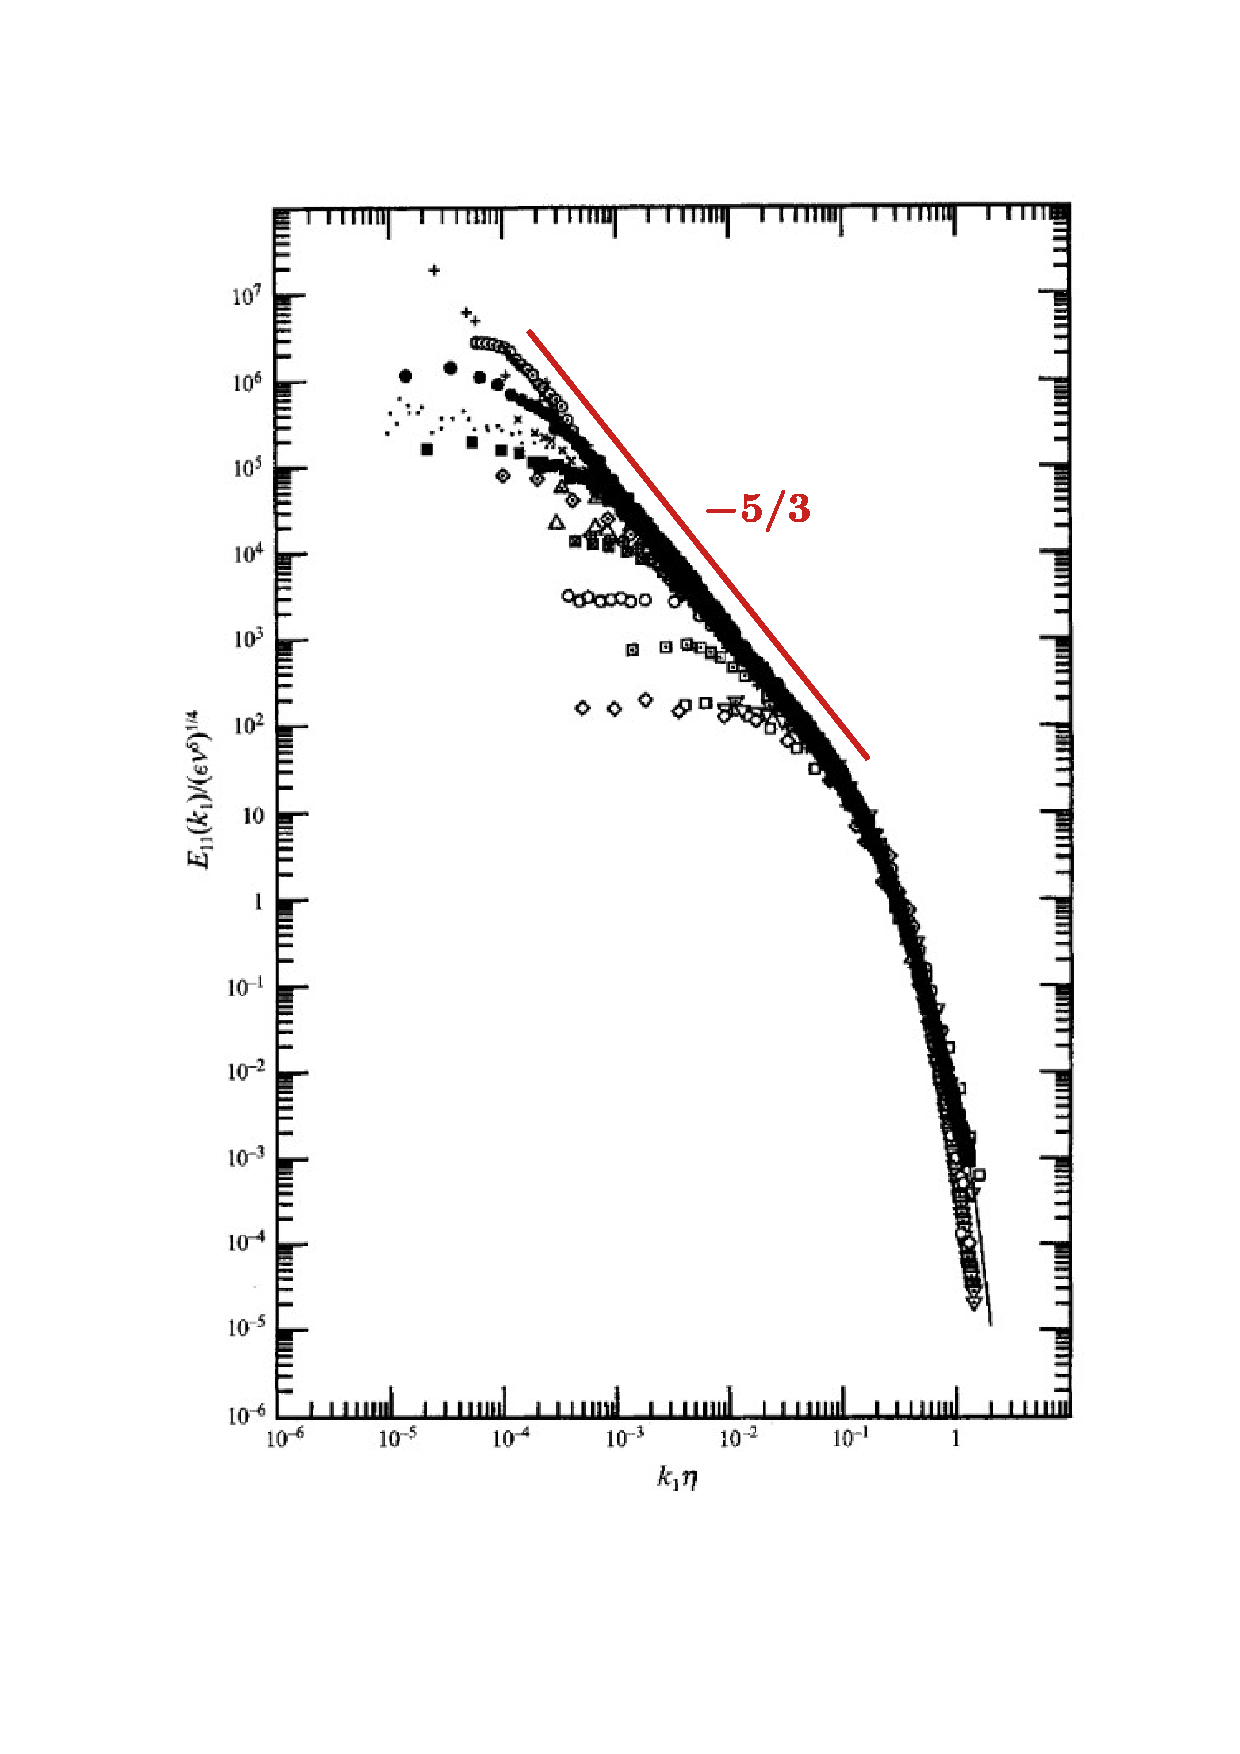
\includegraphics[width=0.8\linewidth,trim=1cm 4cm 1cm 3cm, clip=true]{./Mainmatter/Part_0/images/spectre_kolmogorov}
 \caption{Compilations de spectres obtenus dans diverses expériences de laboratoire. Tous ces spectres sont en accord avec la pente en $-5/3$ prédite grâce à la théorie de Kolmogorov. [Crédits : \cite{saddoughi_local_1994}.] }
 \label{fig:spec_kolmo}
 \end{figure}
 La forme $E(k) = C k^{\gamma}$ avec $C$ et $\gamma$ constants, qui s'écrit  en représentation logarithmique $\log E(k) = \gamma \log k + C $, est une loi d'échelle. Dans un système physique, une loi d'échelle ne va apparaître que sur une gamme d'échelle dédiée, limitée par la taille du système et l'émergence de phénomènes diffusifs à petites échelles, c'est à dire petits $\ell$ ou grands $k$. Ici, cette gamme est la zone de validité de la loi de Kolmogorov : la zone inertielle. 
 
 Cette définition spectrale de la zone inertielle turbulente, telle que le spectre affiche une loi d'échelle en $-5/3$, n'est pas aussi contraignante que la définition statistique via un taux $\varepsilon$ constant. En effet, le système vérifiera plus facilement la définition spectrale que la définition statistique car $E(k)$ est d'ordre 2 ($\propto (\delta v)^2$ et positif) alors que $\varepsilon$ est d'ordre 3 ($\propto (\delta v)^3$ et signé). Autrement dit, observer une pente $-5/3$ de type Kolmogorov ne sera pas forcément synonyme d'un régime de turbulence complètement développée définie par l'existence d'une zone inertielle telle que $\varepsilon$ constant. 
 
 \section{Synthèse des hypothèses de Kolmogorov et de la description de la cascade turbulente via des lois exactes}
 \label{synt-01}
 \fcolorbox{blue}{white}{\begin{minipage}[c]{\linewidth}
  \paragraph{Taux énergétiques échelles-dépendants : }
  \begin{itemize}
      \item Taux de cascade (transfert non linéaire entre les échelles) : $\varepsilon_{NL}(\boldsymbol{\ell})$,
      \item Taux d'injection (forçage) : $\varepsilon_{F}(\boldsymbol{\ell})$,
      \item Taux de dissipation : $\varepsilon_{D}(\boldsymbol{\ell})$.
  \end{itemize}
 
 \paragraph{Loi zéroième ou anomalie dissipative : } $\varepsilon_{D}(\boldsymbol{\ell}= 0) \xrightarrow[\nu \rightarrow 0]{} - \varepsilon \neq 0$. \\$\varepsilon$ correspond au taux de dissipation turbulent.
 
 \paragraph{Méthode d'obtention d'une loi exacte : }
 \begin{itemize}
     \item Dériver l'évolution temporelle d'une fonction de corrélation $\mathcal{R}$ entre deux points indépendants $\mathbf{x}$ et $\mathbf{x'}$ séparés de l'échelle $\boldsymbol{\ell}$, 
     \item Prendre en compte l'hypothèse d'homogénéité statistique, \\ $\Rightarrow$ Loi exacte de type \cacro{KHM}
     \item Appliquer les hypothèses de Kolmogorov de stationarité statistique et séparation d'échelle $\Rightarrow$ Loi exacte de type \cacro{K41}
 \end{itemize}
 
 \paragraph{Propriété liée à l'hypothèse d'homogénéité statistique : } 
 \begin{equation*}
     \Rightarrow \nabla_{\boldsymbol{\ell}}\left<.\right> = \left<\nabla' .\right> = - \left<\nabla . \right>
 \end{equation*}
 
 \paragraph{Propriété liée à l'hypothèse de stationnarité statistique : } $\Rightarrow \partial_t \left<.\right> = 0$.
 
 \paragraph{Hypothèse de séparation d'échelle : } Séparation des gammes d'échelles d'injection/forçage, de cascade/inertielles, et de dissipation/chauffage permise par la loi zéroième.
 \begin{equation*}
 \Rightarrow  \varepsilon_{NL}(0 \ll \boldsymbol{\ell} \ll \boldsymbol{\ell_F} ) = - \varepsilon_{F}(\boldsymbol{\ell} \ll \boldsymbol{\ell_F} ) = \varepsilon_{D}(\boldsymbol{\ell}=0) = - \varepsilon
 \end{equation*}
 
 \paragraph{Loi exacte de type KHM : } $\partial_t \mathcal{R} = \varepsilon_{NL} + \varepsilon_{F} + \varepsilon_{D}$
 
 \paragraph{Loi exacte de type K41 : } $\varepsilon = -\varepsilon_{NL}$
\end{minipage}}

\chapter{Qu'est-ce qu'un plasma ? De l'exemple du vent solaire à la problématique d'étude}
\renewcommand\partie{\Partie\ Chapitre \thechapter}
\label{ch-02}

%\medskip
\minitoc  

\bigskip

Dans le Chapitre \ref{ch-01}, nous avons défini de manière hydrodynamique (HD) ce qu'est la turbulence grâce à la théorie des lois exactes de Kolmogorov. Ce sera le seul chapitre placé dans le domaine hydrodynamique. Dans l'univers visible (ou baryonique), la matière est majoritairement sous forme de plasma que l'on ne peut décrire par les équations de Navier-Stockes incompressibles seules. On s'intéressera donc à la turbulence dans un plasma. 

Ici, nous allons définir ce qu'est un plasma et comment le décrire, puis nous aborderons les questions ouvertes, motivations des travaux décrits dans ce mémoire. 

\section{Les plasmas, état de la matière} \label{sec-021}

La matière peut être décrite comme des poupées russes constituées de particules de tailles diverses, allant des atomes et molécules aux quarks en passant par les protons et les électrons qui sont des particules chargées positivement et négativement. Elle peut aussi être décrite en fonction de son état : solide, liquide, gaz et plasma. 

Les états solide, liquide et gaz sont les états les plus reconnus dans notre quotidien. Ils sont généralement constitués de molécules ou d'atomes neutres ne portant pas de charge électrique. Pourtant, ces états sont des exceptions dans l'univers, où la matière est majoritairement à l'état de plasma : les atomes y sont dissociés en particules chargées, ions, protons et électrons. Ces particules induisent un champ électromagnétique s'il n'y en a pas originellement. Le plasma sera entretenu par les interactions entre les champs électrique et magnétique et les particules. \textbf{\emph{Un plasma est donc un milieu constitué de particules chargées et de champs électrique et magnétique en étroite interaction.}}

On peut aussi en reconnaître dans notre quotidien, le plus souvent ils brillent ! Par exemple, les éclairs, les aurores, les flammes, les néons, les étoiles et les nébuleuses. Ils forment finalement la grande majorité de la matière présente dans l'univers, du centre des planètes au milieu intergalactique. Pour les étudier, on a deux possibilités : les créer en laboratoire ou s'immerger dedans. Dans le deuxième cas, peu sont réellement accessibles, beaucoup étant trop furtif (les éclairs), trop lointains (les nébuleuses) ou trop extrêmes (le soleil) pour y envoyer des appareils de mesure. Parmi les plasmas naturels accessibles, l'espace interplanétaire est roi. Véritable laboratoire [\cite{bruno_solar_2005}], on y envoie régulièrement des sondes et satellites. La dernière sonde en date est \ac{JUICE} lancée le 14 avril 2023 en direction du système lunaire de Jupiter. 

Dans l'espace interplanétaire, on trouve différents types de plasmas. Si l'on décolle de la surface d'une planète telle que la Terre, on commencera par traverser l'atmosphère constituée de gaz neutre. Puis, on atteindra l'ionosphère, un plasma d'ions lourds et impactés par le champ magnétique planétaire. En s'écartant un peu plus, on s'immergera dans la magnétosphère constituée d'ions légers (principalement des protons) et d'électrons, toujours sous l'influence du champ planétaire. En partant du Soleil, on peut aussi définir différentes couches, la chromosphère, une couche fine gazeuse, puis la couronne solaire, un plasma s'étendant sur une quinzaine de rayons solaires et enfin l'héliosphère dans lequel baignent les planètes. Le Soleil y éjecte continuellement un plasma : le vent solaire.
Le mouvement des planètes dans le vent solaire vient former un arc de choc les précédant. Entre cet arc et la magnétosphère, le vent solaire est choqué. Cette région, dominée par le champ magnétique interplanétaire, est la magnétogaine. La \figref{fig:régions} illustre quelques-unes de ces différentes régions. D'autres régions plus spécifiques existent, mais on se contentera de ce niveau de description, le vent solaire étant notre principal objet d'étude. 
\begin{figure}[!ht]
 \centering
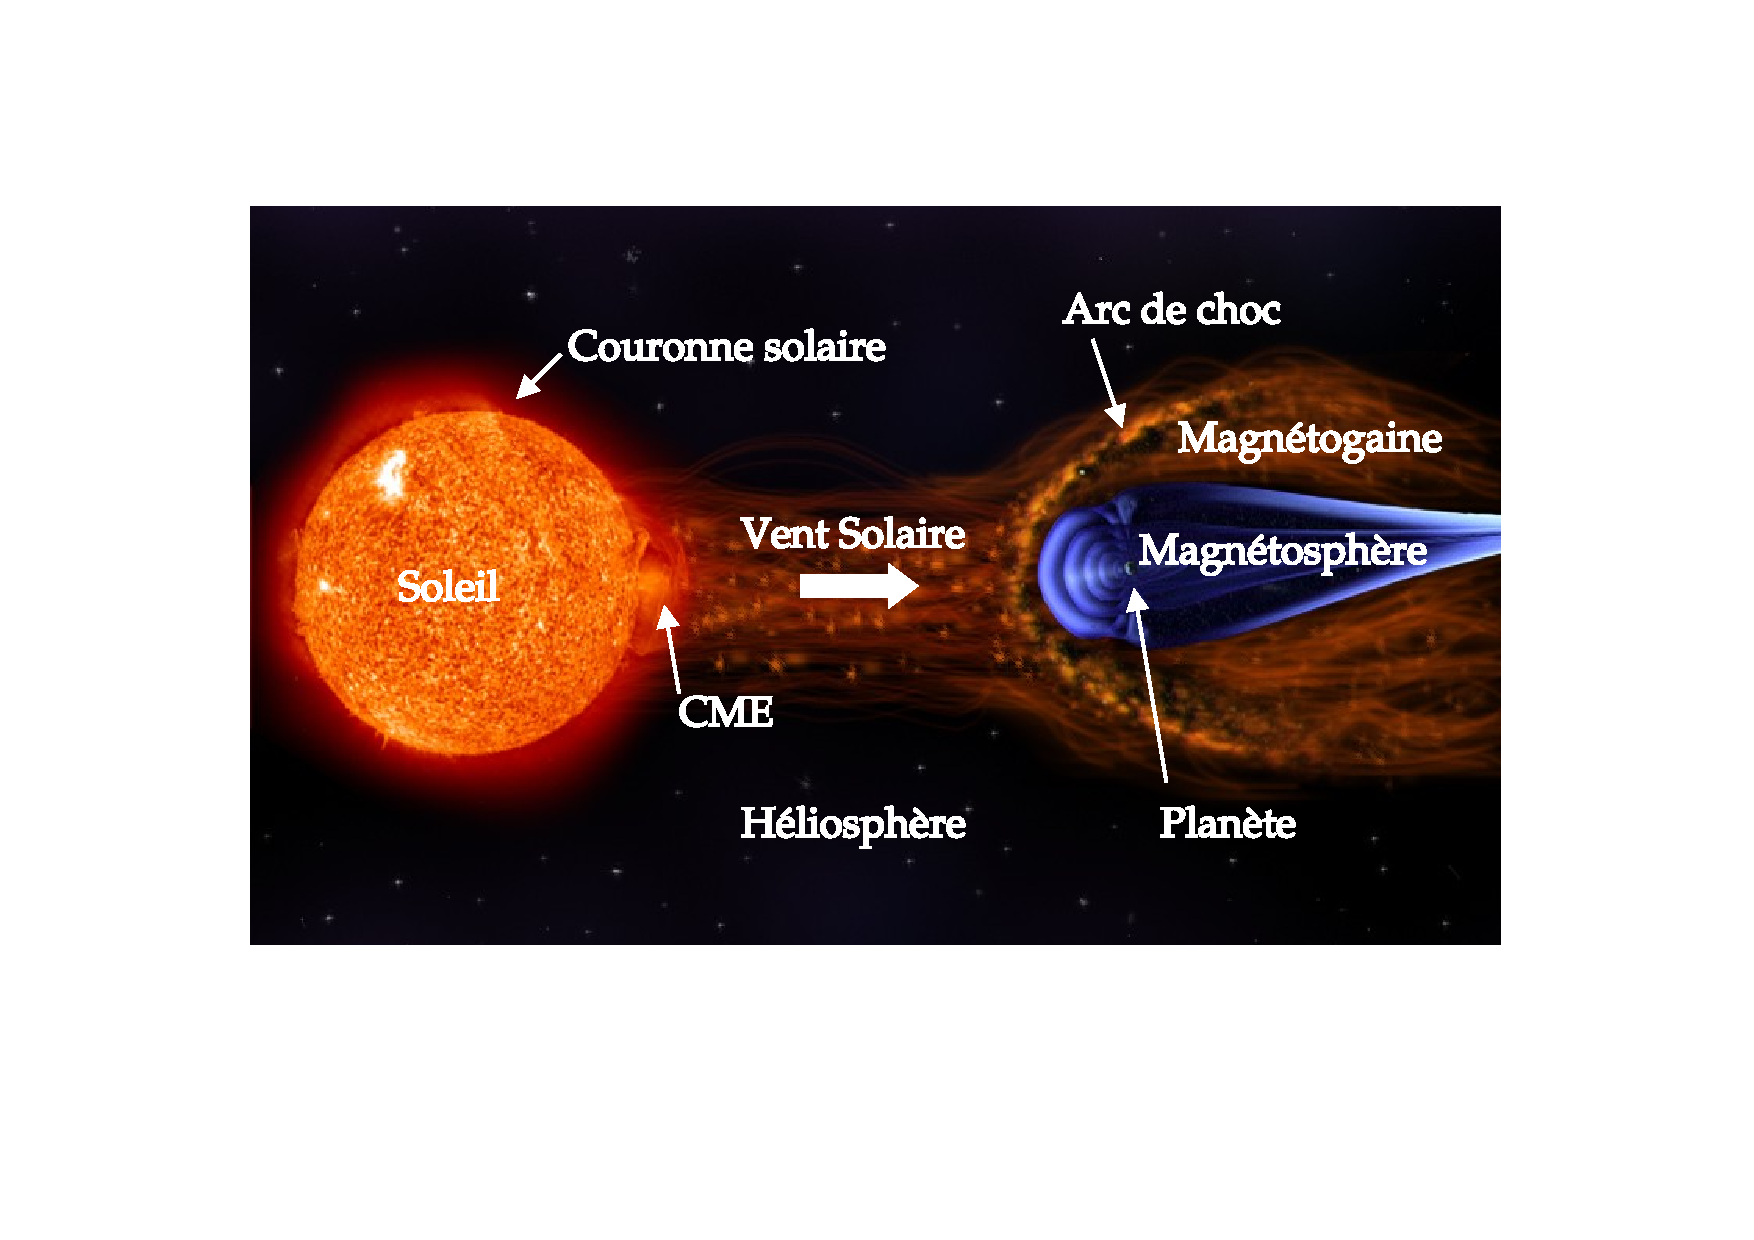
\includegraphics[width=\linewidth,trim=4cm 5cm 4cm 4cm, clip=true]{./Part_0/images/schemes_heliosphere}
\cprotect\caption{Exemples de plasmas spatiaux. \acs{CME} signifie éjections de masse coronale. Crédits de l'image initiale : Institut royal d'Aéronomie Spatiale de Belgique (page web \verb|www.aeronomie.be|).}
\label{fig:régions}
\end{figure}
Le vent solaire est par exemple traversé par \ac{PSP} en orbite autour du Soleil, cette mission lancée par l'agence spatiale américaine \acs{NASA} en 2018 s'approche petit à petit du Soleil afin de <<toucher>> la couronne. La mission \ac{MMS} en orbite autour de la Terre explore le vent solaire, la magnétogaine et la magnétosphère. Nous reparlerons plus en détail de ces deux missions dans le Chapitre \ref{ch-14}. 

\section{Le vent solaire, source de questions ouvertes et problématique d'étude} \label{sec-022}

Le vent solaire est un plasma extrêmement dilué, peu collisionnel et turbulent, constitué essentiellement d'ions légers ou protons (hydrogène, hélium chargés) et d'électrons interagissant avec le champ magnétique du Soleil. En fonction de l'activité cyclique et des latitudes du Soleil, il peut être rapide ($v_{SW} \sim \SI{800}{km/s}$) ou lent ($v_{SW} \sim \SI{400}{km/s}$) et parcouru par des structures à grandes échelles telles que les \ac{CME}. Les missions Voyager 1 et 2, lancées en 1977 vers les confins de l'héliosphère par la NASA, ont permis de tracer les profils de température, champ magnétique, vitesse etc. en fonction de la distance au Soleil [\cite{richardson_radial_1995}]. Ces profils ont donné lieu à diverses modélisations et à des problèmes ouverts encore aujourd'hui. 

\begin{figure}[!ht]
 \centering
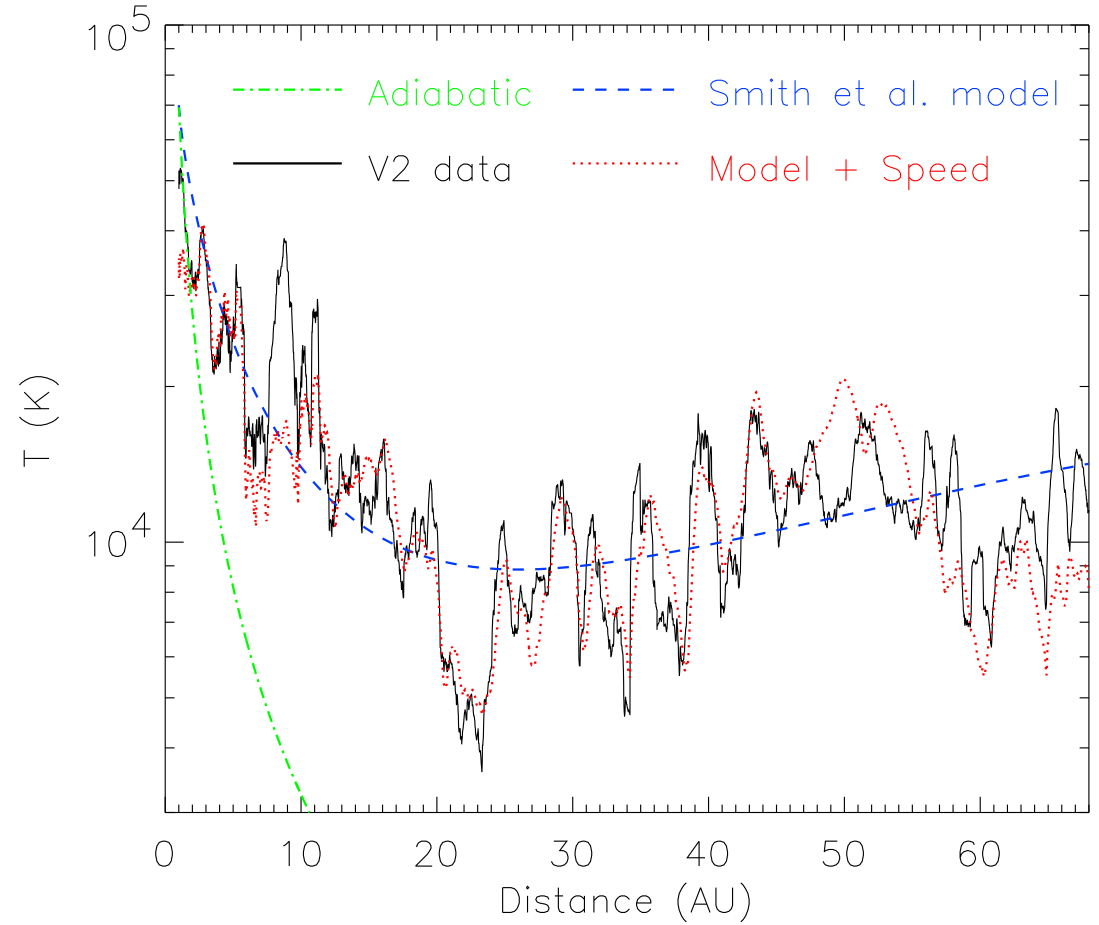
\includegraphics[width=0.8\linewidth,trim=0.5cm 0cm 0cm 0cm, clip=true]{./Part_0/images/heating_profil}
\cprotect\caption{Profil de température ionique en fonction de la distance au Soleil, observé avec les données de Voyager 2 (noir). Profil adiabatique (vert).  Crédits : [\cite{richardson_radial_2003}].}
\label{fig:profil}
\end{figure}
Sur la \figref{fig:profil} est donné l'exemple du profil de température. Du caractère peu collisionnel du vent solaire ont émergé, dans un premier temps, des prédictions d'une décroissance adiabatique du profil de température (courbe verte) [\cite{tu_mhd_1995}]. Comme on peut l'observer, la décroissance n'est pas aussi rapide que le modèle adiabatique. Des exemples de modélisations pour retrouver ce profil sont référencés par [\cite{richardson_radial_2003}]. Sur la \figref{fig:profil}, des résultats d'un modèle prenant en compte des ions dits <<pickups>> sont présentés en bleu et en rouge. Dans le cas rouge, est ajouté au modèle une dépendance linéaire entre la vitesse du vent solaire et la température. Le profil in-situ est ainsi plutôt bien retrouvé mais initialisé à partir de relevés de vitesse et température effectués autour de $\SI{1}{au}$ (unité astronomique dont l'étalon est la distance Soleil-Terre). Les ions pickups font en effet partie des sources du chauffage localisé du vent solaire mais ce chauffage aurait d'autres sources, comme l'explique \cite{david_energy_2022}. 
Avant $\SI{1}{au}$, il serait principalement dû aux fluctuations turbulentes, puis aux chocs interplanétaires venant accélérer ou ralentir le plasma, et enfin, après $\SI{20}{au}$, aux ions pickups provenant du milieu interstellaire. Le chauffage dû aux fluctuations turbulentes est souvent mis en compétition avec un chauffage induit par les processus de reconnexion des lignes de champ magnétique [\cite{matthaeus_who_2011,cranmer_role_2015}]. Ces deux phénomènes sont souvent liés [\cite{sundkvist_dissipation_2007,retino_situ_2007,servidio_magnetic_2011,chasapis_thin_2015,manzini_subion-scale_2023}].  

Dans ces travaux, on s'intéresse au chauffage turbulent [\cite{tu_mhd_1995,kiyani_dissipation_2015}] prédominant à partir de quelques rayons solaires jusqu'à $\SI{2}{au}$. Une définition thermodynamique de ce chauffage sera donnée dans le Chapitre \ref{ch-12}. Ce problème sera abordé à travers la cascade turbulente définie dans le Chapitre \ref{ch-01} et décrite avec une théorie des lois exactes, héritage de la théorie de Kolmogorov. Elle permet un transfert d'énergie des grandes échelles d'injection, à travers les échelles dites fluides et vers les petites échelles (échelles dites cinétiques) où les processus cinétiques dissipatifs peuvent intervenir afin de chauffer les ions et les électrons. 

Ce transfert peut être illustré à partir des spectres d'énergie magnétique comme celui de la \figref{fig:spectre_SW} compilé grâce aux relevés de champ magnétique effectués in-situ par les missions \ac{ACE} et \acs{CLUSTER} en orbite autour de la Terre.  Sur cette figure, on retrouve en fonction de la fréquence temporelle $f$ une pente de type Kolmogorov en $-5/3 \simeq -1.7$. L'hypothèse de Taylor permet de relier le vecteur d'onde $\boldsymbol{k}$ introduit dans le Chapitre \ref{ch-01}, à la fréquence temporelle $f$ accessible dans les relevés in-situ, grâce à la vitesse du vent ($\boldsymbol{v}_{SW}$) : $2 \pi f \sim \boldsymbol{v}_{SW} \cdot \boldsymbol{k}$.
Cette pente indique donc les échelles inertielles et la présence de turbulence dans le plasma d'après la définition spectrale de la zone inertielle donnée dans le Chapitre \ref{ch-01} et transposée à l'énergie magnétique. 
À plus hautes fréquences, cette zone inertielle s'achève par une rupture de pente autour de la fréquence associée à une longueur caractéristique ionique (la longueur d'inertie ($d_i$) ou le rayon de Larmor ($\rho_{Li}$) noté sur la figure $\rho_i$). 
À partir de cette échelle, des effets cinétiques ioniques commencent donc à être visibles. Ensuite, le spectre semble se stabiliser autour d'un nouveau régime a priori dispersif, avec une pente proche de $-2.6$, avant d'atteindre la zone d'influence des électrons autour de la fréquence associée à une longueur caractéristique électronique ($d_e$ ou $\rho_{Le}$, noté sur la figure $\rho_e$). Les phénomènes d'origine cinétique impliqués dans la zone de transition et les zones qui s'ensuivent ne sont pas encore complètement compris, tout comme leurs impacts sur les régimes turbulents (voir par exemple \cite{alexandrova_solar_2013} et \cite{sahraoui_magnetohydrodynamic_2020}). 
\begin{figure}[!ht]
 \centering
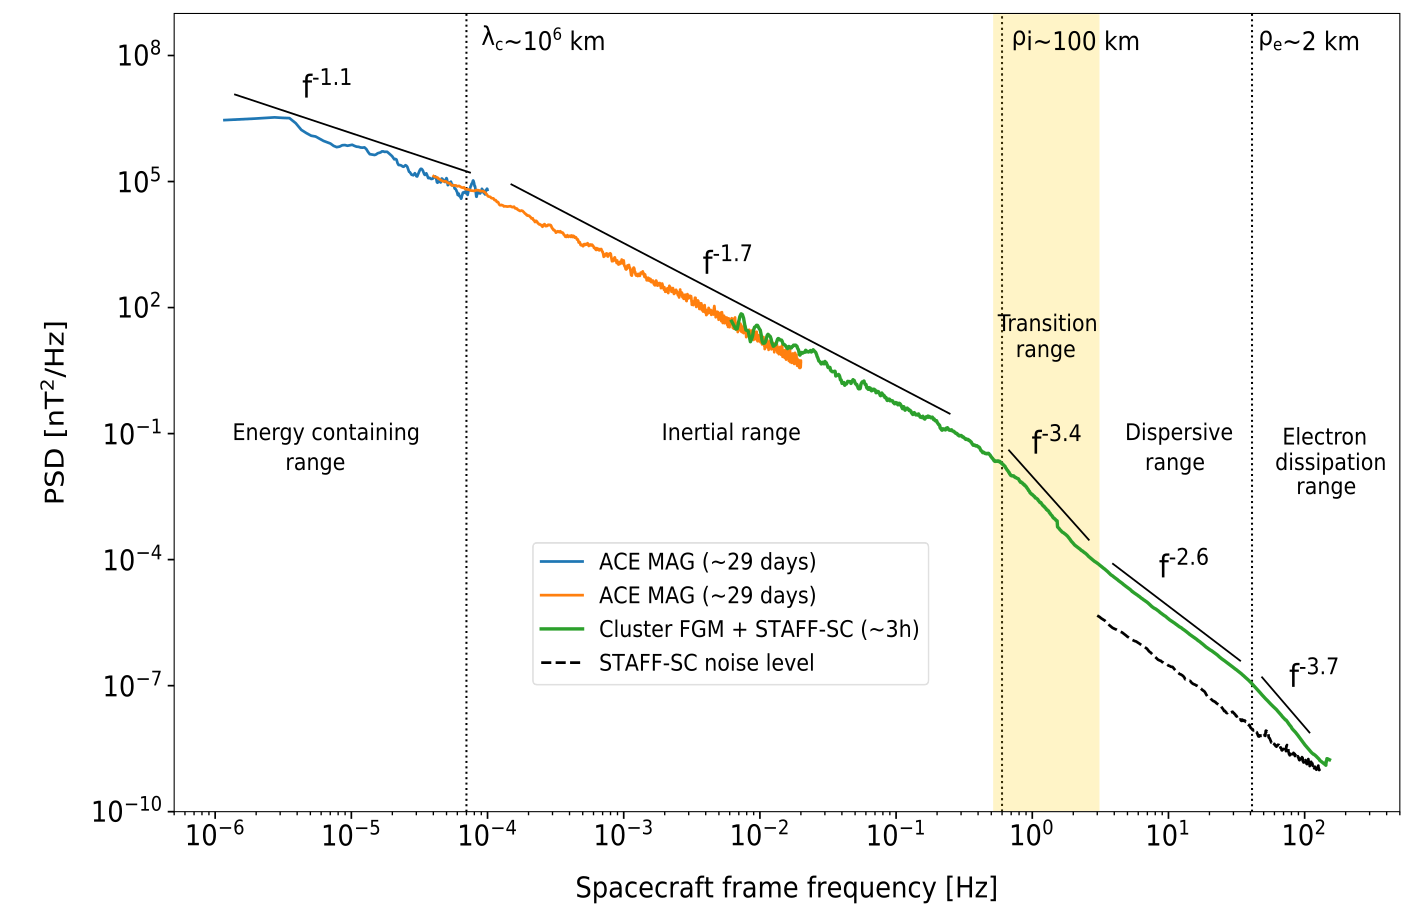
\includegraphics[width=\linewidth,trim=0.5cm 0cm 0cm 0cm, clip=true]{./Part_0/images/spectre_SW}
\cprotect\caption{Spectre d'énergie magnétique du vent solaire obtenu à partir des missions ACE et Cluster. Ce spectre peut être découpé en cinq régions grâce aux ruptures de pentes. Pente en $-1.1$ : Réservoir d'énergie. $\lambda_c$ : longueur de corrélation. Pente en $-1.7$ : Zone inertielle. $\rho_i$ : rayon de Larmor ionique. Pente en $-3.4$ : Zone de transition. Pente en $-2.6$ : Échelles dispersives. $\rho_e$ : rayon de Larmor électronique. Pente en $-3.7$ : Échelles de dissipation électronique. Crédits : [\cite{sahraoui_magnetohydrodynamic_2020}].}
\label{fig:spectre_SW}
\end{figure}

Parmi ces questions ouvertes dans l'étude de la turbulence compressible pour le chauffage du vent solaire, on s'attaquera aux effets conjoints du manque de collision et du champ magnétique sur la cascade. Ces deux propriétés induisent une anisotropie de la fonction de distribution de vitesse des particules, menant à un tenseur de pression anisotrope. Cette anisotropie de pression peut induire des instabilités dans le système [\cite{parker_dynamical_1958,berezin_firehose_1976,hall_firehose_1981,southwood_mirror_1993,gary_proton_1976,hunana_introductory_2019}]. 

La cascade turbulente d'énergie a été largement étudiée dans le cas incompressible depuis le début du siècle et l'extension de la théorie des lois exactes de Kolmogorov au modèle magnétohydrodynamique incompressible par \cite{politano_von_1998} et \cite{politano_dynamical_1998}. Les études sur l'effet de la compression sur la cascade sont quant à elles plus récentes et leur cadre souvent limité par l'hypothèse thermodynamique isotherme [\cite{marino_scaling_2023}]. Dans le Chapitre \ref{ch-11}, nous reprendrons quelques résultats incompressibles avant d'apporter dans la Partie \ref{part_1} une première extension du cadre d'étude de la cascade turbulente à des plasmas compressibles, en centrant la problématique sur l'effet de différentes descriptions thermodynamiques utilisées pour définir la pression. Dans la Partie \ref{part_2}, nous élargirons le cadre de la théorie des lois exactes en prenant en compte l'anisotropie de pression. Dans la Partie \ref{part_3}, nous appliquerons la théorie analytique ainsi élargie à des simulations tridimensionnelles turbulentes. 

Mais, avant cela, dans la section \ref{sec-023}, sera rappelée la description fluide d'un plasma qui sert de base à l'ensemble des modèles utilisés dans ces travaux, et, dans le Chapitre \ref{ch-11}, nous allons introduire la première extension de la théorie de Kolmogorov à un plasma et quelques résultats fondamentaux associés aux plasmas incompressibles. 

\section{Décrire un plasma à l'aide d'un modèle fluide} \label{sec-023}

Soit un plasma, dans lequel chaque particule est caractérisée par le ratio charge/masse, $q_{\alpha}/m_{\alpha}$, associée à son espèce notée $\alpha$, sa position dans l'espace des phases $\{\mathbf{x},\mathbf{v}\}$ et une fonction de distribution $\mathcal{P}_{\alpha}\left(\mathbf{x},\mathbf{v},t\right)$. Dans les cas étudiés ici, les espèces sont les protons ($\alpha = i$) et les électrons ($\alpha=e$). En négligeant les collisions entre les particules, l'équation cinétique, nommée alors équation de Vlasov, décrivant l'évolution de la fonction de distribution des particules est : 
\begin{equation}
\partial_t \mathcal{P}_{\alpha} +  \mathbf{v} \cdot \nabla \cdot \mathcal{P}_{\alpha} + \frac{d \mathbf{v}}{d t} \cdot \nabla_{\mathbf{v}}  \cdot  \mathcal{P}_{\alpha}  = 0.
\label{kinetic vlasov}
\end{equation}
Le système est alors décrit par sept variables, une temporelle $t$, les trois composantes de la position $\mathbf{x}=\left[x,y,z\right]$ associée à l'opérateur dérivatif $\nabla$ et les trois composantes de la vitesse $\mathbf{v}$ associée à l'opérateur dérivatif $\nabla_{\mathbf{v}}$ et dépendante du temps. Si l'on considère que les particules baignent dans un champ électromagnétique $\{\boldsymbol{E}\left(\mathbf{x},t\right),\boldsymbol{B}\left(\mathbf{x},t\right)\}$, on peut remplacer $\frac{d \mathbf{v}}{d t}$  par la force électromagnétique de Lorentz $q_{\alpha}/m_{\alpha} \left(\boldsymbol{E} + \mathbf{v} \times \boldsymbol{B}\right)$ et compléter le système avec les équations de Maxwell :
\begin{eqnarray}
    \label{eq:M1}\nabla \cdot \boldsymbol{E} &=& Q/\epsilon_0 ,\\
     \label{eq:M2}\nabla \cdot \boldsymbol{B} &=& 0 ,\\
     \label{eq:M3}\nabla \times \boldsymbol{E} &=& -\partial_t \boldsymbol{B} ,\\
     \label{eq:M4}\nabla \times \boldsymbol{B} &=& \mu_0 \boldsymbol{j} + \epsilon_0 \mu_0 \partial_t \boldsymbol{E} ,
\end{eqnarray}
avec $Q\left(\mathbf{x},t\right)$ et  $\boldsymbol{j}\left(\mathbf{x},t\right)$ les densités totales de charges et de courant du plasma. 

On peut définir des quantités macroscopiques, des <<moments>> de la fonction de distribution, en moyennant une fonction $g\left(\mathbf{x},\mathbf{v},t\right)$ dans l'espace des vitesses ($d^3v=dv_xdv_ydv_z$) : 
\begin{equation}
 \left<G\left(\mathbf{x},t\right)\right>_{\alpha} = \int^{+\infty}_{-\infty} \mathcal{P}_{\alpha}\left(\mathbf{x},\mathbf{v},t\right) g\left(\mathbf{x},\mathbf{v},t\right) d^3v \, .
\end{equation}
Afin d'appliquer cette moyenne, on supposera la convergence des intégrales. Les étapes de calculs ne seront pas détaillées. Pour plus d'informations, se référer à, par exemple, [\cite{krall_principles_1973,rax_physique_2005,galtier_introduction_2016,belmont_introduction_2018}].
Visuellement, les moments d'ordre 0, sont reliés à l'aire sous la fonction de distribution, ceux d'ordre 1 sont reliés à sa valeur moyenne et ceux d'ordre 2 à sa largeur à mi-hauteur comme représenté sur la \figref{fig:distrib}. 
\begin{figure}[!ht]
 \centering
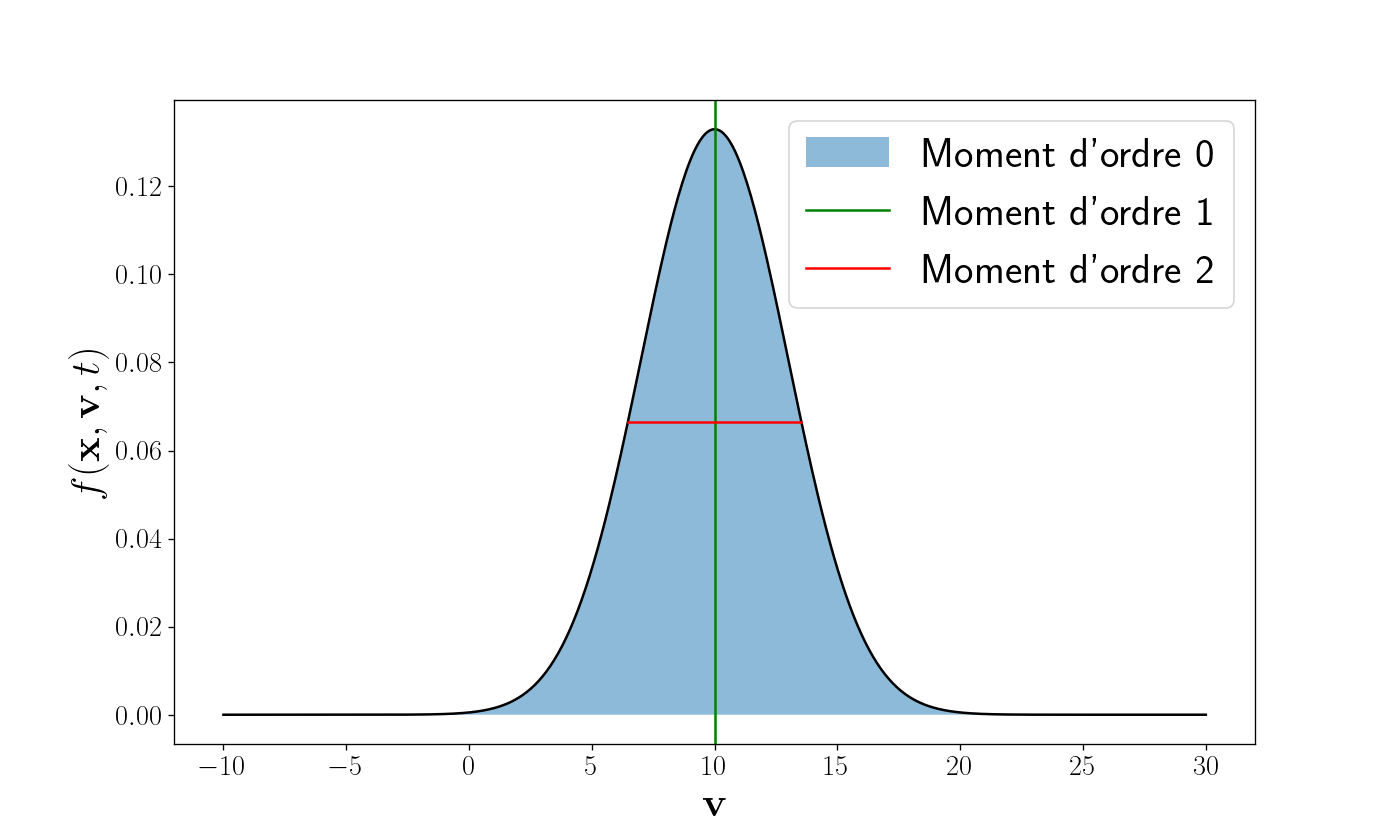
\includegraphics[width=\linewidth,trim=2cm 0cm 3cm 1cm, clip=true]{./Part_0/images/distrib}
\cprotect\caption{Représentation graphique des moments d'ordre 0 (aire sous la courbe colorée en bleu), 1 (valeur moyenne de $\mathbf{v}$ indiquée par la verticale verte) et 2 (largeur indiquée par l'horizontale rouge) de la fonction de distribution en vitesse $f\left(\mathbf{x},\mathbf{v},t\right)$ ici gaussienne.}
\label{fig:distrib}
\end{figure}
 

Suivant la fonction $g$, on peut obtenir pour chaque espèce, les quantités macroscopiques suivantes, aussi appelées <<moments>>,  : 
\begin{table}[!ht]
\begin{center}
\begin{tabular}{ c|c|c|c } 
Quantité & $\left<G\left(\mathbf{x},t\right)\right>_{\alpha}$ & $g\left(\mathbf{x},\mathbf{v},t\right)$  & ordre\\
\hline
Densité de particules & $n_{\alpha}\left(\mathbf{x},t\right)$ & $1$  & 0 \\
Densité de masse & $\rho_{\alpha}\left(\mathbf{x},t\right)$ & $m_{\alpha}\left(\mathbf{x},t\right)$ & 0 \\
Densité de charge & $Q_{\alpha}\left(\mathbf{x},t\right)$ & $q_{\alpha}\left(\mathbf{x},t\right)$ & 0\\
Densité de vitesse du fluide & $n_{\alpha} \boldsymbol{v_{\alpha}}\left(\mathbf{x},t\right)$ & $\mathbf{v}$ & 1\\
Densité de courant & $\boldsymbol{j_{\alpha}}\left(\mathbf{x},t\right)$ & $q_{\alpha} \boldsymbol{v_{\alpha}}$ & 1\\
Pression & $\overline{\boldsymbol{P_{\alpha}}} \left(\mathbf{x},t\right)$ & $m_{\alpha}\left(\mathbf{v}-\boldsymbol{v_{\alpha}}\right)\left(\mathbf{v}-\boldsymbol{v_{\alpha}}\right)$ & 2\\
Flux de chaleur& $\overline{\overline{\boldsymbol{q_{\alpha}}}}\left(\mathbf{x},t\right)$ & $m_{\alpha}\left(\mathbf{v}-\boldsymbol{v_{\alpha}}\right)\left(\mathbf{v}-\boldsymbol{v_{\alpha}}\right)\left(\mathbf{v}-\boldsymbol{v_{\alpha}}\right)$ & 3\\
\end{tabular}
\end{center}
\end{table}

À partir de l'équation de Vlasov, on obtient des équations dites <<multi-fluides>> (dépendantes de $\alpha$) décrivant l'évolution des différents moments :
\begin{itemize}
    \item L'équation de continuité pour la densité massique :
\begin{eqnarray}
  \label{eq:model_0_multi} \partial_t \rho_{\alpha} + \nabla \cdot \left(\rho_{\alpha} \boldsymbol{v_{\alpha}}\right) &=& 0.
 \end{eqnarray}
    \item L'équation sur la quantité de mouvement :
\begin{eqnarray}
  \label{eq:model_1_multi} \partial_t \left(\rho_{\alpha} \boldsymbol{v_{\alpha}}\right) + \nabla \cdot \left(\rho_{\alpha} \boldsymbol{v_{\alpha}}\boldsymbol{v_{\alpha}} + \overline{\boldsymbol{P_{\alpha}}}\right) - Q_{\alpha} \boldsymbol{E} - \boldsymbol{j_{\alpha}} \times \boldsymbol{B} &=& 0.
 \end{eqnarray}
 \item L'équation d'évolution du tenseur de pression :
\begin{eqnarray}
  \label{eq:model_2_multi} \partial_t \overline{\boldsymbol{P_{\alpha}}} + \nabla \cdot \left(\boldsymbol{v_{\alpha}}\overline{\boldsymbol{P_{\alpha}}} + \overline{\overline{\boldsymbol{q_{\alpha}}}}\right) + \left(\overline{\boldsymbol{P_{\alpha}}} \cdot \nabla \boldsymbol{v_{\alpha}}\right)^S +  \frac{Q_{\alpha}}{\rho_{\alpha}} \left(\boldsymbol{B}\times \overline{\boldsymbol{P_{\alpha}}}\right)^S  &=& 0 ,
\end{eqnarray}
\end{itemize}
avec $\left( \right)^S = \left( \right) + \left( \right)^T$ avec $\left( \right)^T$ la transposée de $\left( \right)$. Ces équations sont associées respectivement aux moments d'ordre 0, 1 et 2. On remarque que l'équation du moment d'ordre $n$ dépend d'un moment d'ordre $n+1$. Afin de fermer le système d'équations, des équations dites <<de fermeture>>, devront être introduites. 

Dans les plasmas que l'on considère, on a deux populations ($\alpha = i,e$): les ions/protons ($m_i$, $e$) et les électrons ($m_e$, $-e$) avec les masses $m_i \gg m_e$ et $e$ la charge élémentaire. Le système d'équation multi-fluide sera donc appelé <<bi-fluide>>. On l'abordera dans le Chapitre \ref{ch-23}. 

Les quantités totales (notées sans indices : $n$, $\rho$, $\boldsymbol{v}$, $\boldsymbol{j}$, etc.) sont ensuite obtenues en sommant sur toutes les espèces, $n_{\alpha}$, $\rho_{\alpha}$, $Q_{\alpha}$, $\rho_{\alpha} \boldsymbol{v_{\alpha}}$, $\boldsymbol{j_{\alpha}}$, $\overline{\boldsymbol{P_{\alpha}}} +  \rho_{\alpha} \boldsymbol{v_{\alpha}}\boldsymbol{v_{\alpha}}$ et $\rho_{\alpha} u_{\alpha} + \frac{1}{2} \rho_{\alpha} |\boldsymbol{v_{\alpha}}|^2$.  En appliquant ces sommations aux équations \eqref{eq:model_0_multi}, \eqref{eq:model_1_multi} et \eqref{eq:model_2_multi} et en considérant l'hypothèse de quasi-neutralité ($Q \simeq 0$), on obtient les équations mono-fluides quasi-neutres suivantes :
\begin{itemize}
    \item L'équation de continuité pour la densité massique :
\begin{eqnarray}
  \label{eq:model_0_mono} \Rightarrow \partial_t \rho + \nabla \cdot \left(\rho \boldsymbol{v}\right) &=& 0 .
 \end{eqnarray}
    \item L'équation sur la quantité de mouvement :
\begin{eqnarray}
\label{eq:model_1_mono} \Rightarrow \partial_t \left(\rho \boldsymbol{v}\right) + \nabla \cdot \left(\rho \boldsymbol{v}\boldsymbol{v} + \overline{\boldsymbol{P}}\right) - \boldsymbol{j} \times \boldsymbol{B} &=& 0 .
 \end{eqnarray}
 \item L'équation d'évolution du tenseur de pression, avec $\overline{\boldsymbol{P_E}} = \sum_{\alpha} \frac{Q_{\alpha}}{\rho_{\alpha}} \overline{\boldsymbol{P_{\alpha}}}$ :
\begin{eqnarray}
 \label{eq:model_2_mono} \Rightarrow \partial_t \overline{\boldsymbol{P}} + \nabla \cdot \left(\boldsymbol{v}\overline{\boldsymbol{P}} + \overline{\overline{\boldsymbol{q}}}\right) + \left(\overline{\boldsymbol{P}} \cdot \nabla \boldsymbol{v}\right)^S +  \frac{Q}{\rho} \left(\boldsymbol{B}\times \overline{\boldsymbol{P_E}}\right)^S  &=& 0 .
\end{eqnarray}
\end{itemize}
L'hypothèse non-relativiste et la quasi-neutralité permettent d'y remplacer $\boldsymbol{j}$ par $\nabla \times \boldsymbol{B}$ (Equation de Maxwell \eqref{eq:M4}).

On peut construire, à partir de l'équation \eqref{eq:model_1_multi}, l'équation d'évolution de la densité de courant totale $\boldsymbol{j} = e n_i \boldsymbol{v_i} - e n_e \boldsymbol{v_e}$. Sachant que $m_i \gg m_e$, cette équation peut s'écrire sous la forme de la loi d'Ohm généralisée : \begin{equation} 
\boldsymbol{E} =  \boldsymbol{E_{ind}} +  \boldsymbol{E_{hall}} +  \boldsymbol{E_{therm}} \label{eq:ohm} 
\end{equation}
avec :
\begin{itemize}
 \item $\boldsymbol{E_{MHD}} =  - \boldsymbol{v} \times \boldsymbol{B}$, le terme d'induction,
 \item $\boldsymbol{E_{hall}} = \lambda_i \frac{\boldsymbol{j}}{\rho} \times \boldsymbol{B}$, le terme de \acl{Hall},
 \item $\boldsymbol{E_{\nabla P_e}} = - \frac{\lambda_i}{\rho} \nabla \cdot \overline{\boldsymbol{P_{e}}}$,  \acl{Pe},
\end{itemize}
avec $\lambda_i = \frac{m_i}{e}$. La loi d'Ohm permet d'expliciter $\boldsymbol{E}$ dans l'équation \eqref{eq:M3}. En ne prenant en compte que le terme d'induction dans la loi d'Ohm, on obtient l'équation : 
\begin{equation}
    \label{eq:model_M3_ideal} \partial_t \boldsymbol{B} = \nabla \times \left(\boldsymbol{v} \times \boldsymbol{B} \right)
\end{equation}
qui s'écrit en fonction de la vitesse d'Alfvén $\boldsymbol{v_A} = \frac{\boldsymbol{B}}{\sqrt{\mu_0 \rho}}$ avec $\mu_0$, la perméabilité du vide, : 
\begin{equation}
\label{eq:model_M3_idealvA} \partial_t \boldsymbol{v_A}  =   \nabla \cdot \left(\boldsymbol{v_A}\boldsymbol{v} - \boldsymbol{v}\boldsymbol{v_A}\right) -  \boldsymbol{v}  \nabla \cdot \boldsymbol{v_A} +  \frac{\boldsymbol{v_A}}{2}  \nabla \cdot \boldsymbol{v}. \end{equation}

Les équations \eqref{eq:model_0_mono}, \eqref{eq:model_1_mono} avec l'hypothèse non-relativiste, \eqref{eq:model_2_mono} et  \eqref{eq:model_M3_ideal} forment le modèle \ac{MHD} non fermé, valable pour des échelles temporelles associées à des fréquences plus petites que la fréquence cyclotron ionique $\omega_{ci} = B_0/\lambda_i$ avec $B_0 = \left<|\boldsymbol{B}|\right>$ et des échelles spatiales, dites \ac{MHD}, plus grandes que $d_i$ et $\rho_{Li}$. En fonction de l'équation de fermeture choisie, l'équation \eqref{eq:model_2_mono} peut être omise, par exemple dans le cas d'une fermeture isotherme où $\overline{\boldsymbol{P}} \propto \rho$.
Usuellement, la pression est supposée isotrope dans le modèle \acs{MHD} mais dans ce mémoire, on ne fera cette hypothèse que dans la Partie \ref{part_1}. Dans la Partie \ref{part_2}, on abordera l'extension de la théorie des lois exactes au modèle \acs{MHDH} pour laquelle l'équation d'induction peut s'écrire : 
\begin{equation}
\partial_t \boldsymbol{v_A}  =   \nabla \cdot \left(\boldsymbol{v_A}\boldsymbol{v} - \boldsymbol{v}\boldsymbol{v_A}\right) -  \boldsymbol{v}  \nabla \cdot \boldsymbol{v_A} +  \frac{\boldsymbol{v_A}}{2}  \nabla \cdot \boldsymbol{v} - \frac{\lambda}{ \sqrt{\rho} } \nabla \times\left(\frac{1}{\sqrt{\rho}} \boldsymbol{j}\times \boldsymbol{v_A}\right)  .\label{eq:model_M3_hall}
\end{equation}
Ce modèle est souvent normalisé par la vitesse d'Alfvén moyenne $v_{A0}$. Dans l'équation \eqref{eq:model_M3_hall}, $\lambda_i$ est alors remplacée par la longueur inertielle des ions $d_i = v_{A0}\omega_{ci}$. Ce modèle sera donc valable aux échelles MHD et aux échelles dites Hall, proches de $d_i$. Certaines simulations que l'on analysera dans la Partie \ref{part_3} prennent aussi en compte le \acl{Pe}. Nous proposerons donc une extension au modèle \acs{MHDHPe}. Ce terme permet de prendre en compte la contribution thermique des électrons au champ électrique. 
%Le terme inertiel électronique, dépendant de $\lambda_e$, permet quant à lui d'accéder aux échelles électroniques proches de $d_e$ ou $\rho_{Le}$.

\section{Synthèse : problématique et modèles utilisés}
\label{synt-02}
\fcolorbox{red}{white}{\begin{minipage}[c]{\linewidth}
\paragraph{Problématique générale : } Quel est l'impact des fermetures dépendant de la pression sur la cascade turbulente ? \\

\paragraph{Plan : }
\begin{itemize}
    \item Partie \ref{part_1} : Impact d'une pression isotrope sur la cascade turbulente compressible,
    \item Partie \ref{part_2} : Description d'un écoulement turbulent dépendant d'une pression anisotrope,
    \item Partie \ref{part_3} : Effet de l'anisotropie de pression sur la cascade turbulente. \\
\end{itemize}
\end{minipage}}

\fcolorbox{blue}{white}{\begin{minipage}[c]{\linewidth}

\paragraph{Modèles utilisés}
\begin{eqnarray}
  \label{eq:synth_model_0_mono} \Rightarrow \partial_t \rho + \nabla \cdot \left(\rho \boldsymbol{v}\right) &=& 0 \\
\label{eq:synth_model_1_mono} \Rightarrow \partial_t \left(\rho \boldsymbol{v}\right) + \nabla \cdot \left(\rho \boldsymbol{v}\boldsymbol{v} + \overline{\boldsymbol{P}}\right) - \boldsymbol{j} \times \boldsymbol{B} &=& 0 \\
 \label{eq:synth_model_2_mono} \Rightarrow \partial_t \overline{\boldsymbol{P}} + \nabla \cdot \left(\boldsymbol{v}\overline{\boldsymbol{P}} + \overline{\overline{\boldsymbol{q}}}\right) + \left(\overline{\boldsymbol{P}} \cdot \nabla \boldsymbol{v}\right)^S +  \left(\boldsymbol{B}\times \overline{\boldsymbol{P_E}}\right)^S  &=& 0 
\end{eqnarray}
\begin{itemize}
\item \ac{MHD} (Parties \ref{part_1} et \ref{part_2}) : 
\begin{equation}
    \label{eq:synth_M3_ideal} \partial_t \boldsymbol{B} = \nabla \times \left(\boldsymbol{v} \times \boldsymbol{B} \right)
\end{equation}
\item \acs{MHDH} (Parties \ref{part_2} et \ref{part_3}) : 
\begin{equation}
    \label{eq:synth_M3_hall} \partial_t \boldsymbol{B} = \nabla \times \left(\boldsymbol{v} \times \boldsymbol{B} \right) - \lambda \nabla \times \left( \frac{\boldsymbol{j}}{\rho} \times \boldsymbol{B} \right)
\end{equation}
\item \acs{MHDHPe} (Parties \ref{part_2} et \ref{part_3}) : 
\begin{equation}
    \label{eq:synth_M3_gpe} \partial_t \boldsymbol{B} = \nabla \times \left(\boldsymbol{v} \times \boldsymbol{B} \right) - \lambda \nabla \times \left( \frac{\boldsymbol{j}}{\rho} \times \boldsymbol{B} \right) + \lambda \nabla \times \left( \frac{1}{\rho} \nabla \cdot \overline{\boldsymbol{P_{e}}}\right)
\end{equation}
\item Autre : Bi-fluide (Parties \ref{part_2})\\
\end{itemize}

\end{minipage}}

\chapter{Etude de la cascade turbulente dans un plasma incompressible}
\renewcommand\partie{\Partie\ Chapitre \thechapter}
\label{ch-11}

%\medskip
\minitoc  

\bigskip

Ce n'est que 57 ans après l'apport de Kolmogorov à la compréhension de la turbulence que l'idée de chercher des lois exactes dans un fluide magnétisé, ou plasma, a émergé. Ainsi, \cite{politano_von_1998} et \cite{politano_dynamical_1998} ont étendu la théorie hydrodynamique à la \ac{MHD} en restant dans le cadre incompressible. Cette avancée historique a apporté un cadre à l'étude de la turbulence dans les plasmas spatiaux. Dans le laboratoire qu'est le vent solaire, elle a permis de trouver des éléments de réponse à des problèmes tels que ceux du chauffage ou de l'accélération du vent [\cite{smith_dependence_2006,sorriso-valvo_observation_2007,stawarz_turbulent_2009,osman_proton_2013,bruno_solar_2013,alexandrova_solar_2013,sahraoui_magnetohydrodynamic_2020,marino_scaling_2023}]. 

Le modèle incompressible magnétohydrodynamique idéal avec pression isotrope (\acs{IMHD}) est la description fluide d'un plasma la plus simple abordée dans ce mémoire. Dans ce chapitre, nous reprendrons les résultats analytiques incompressibles principaux afin d'introduire les outils fondamentaux de l'étude de la turbulence dans un plasma.

\section{Le modèle et l'énergie totale}
\label{sec-111}
Contrairement au modèle hydrodynamique incompressible abordé dans le Chapitre \ref{ch-01}, dans le cas d'un plasma, il est nécessaire de prendre en compte le couplage entre le fluide et le champ magnétique et d'ajouter l'équation d'induction \eqref{eq:synth_M3_ideal} comme on a pu le mettre en pratique dans le Chapitre \ref{ch-02}. L'incompressibilité s'exprime quant à elle à travers la contrainte $\nabla \cdot \boldsymbol{v} = 0$. Le modèle magnétohydrodynamique incompressible (\acs{IMHD}) est alors :
\begin{eqnarray}
\label{eq:model_inc_v} \partial_t \boldsymbol{v} + \boldsymbol{v} \cdot \nabla \boldsymbol{v} -  \boldsymbol{v_A} \cdot \nabla \boldsymbol{v_A} + \frac{1}{\rho_0} \nabla p_* &=& 0, \\
\label{eq:model_inc_b} \partial_t \boldsymbol{v_A} + \boldsymbol{v} \cdot \nabla \boldsymbol{v_A} -  \boldsymbol{v_A} \cdot \nabla \boldsymbol{v}&=& 0, \\
\label{eq:model_inc_r} \nabla \cdot \boldsymbol{v} &=& 0.
\end{eqnarray}
Le champ magnétique apparaît dans ces équations à travers la vitesse d'Alfvén $\boldsymbol{v_A} = \boldsymbol{B}/\sqrt{\mu_0 \rho_0}$ et la pression magnétique $p_m = \rho_0 \boldsymbol{v_A}^2 /2$ contenue dans la pression totale $p_* = p + p_m$. On remarque qu'il y a 3 équations (7 en termes de composantes) et 3 inconnues (2 vectorielles, $\boldsymbol{v}$ et $\boldsymbol{v_A}$ et une scalaire, $p$). Le système se retrouve donc fermé grâce à la contrainte incompressible en équation \eqref{eq:model_inc_r}. On peut rappeler aussi que le champ magnétique est aussi contraint tel que $\nabla \cdot \boldsymbol{B} = 0$, ce qui implique dans le cas incompressible : $\nabla \cdot \boldsymbol{v_A} = 0$ (contrainte implicitement prise en compte dans l'équation d'induction \eqref{eq:model_inc_b}). En appliquant la divergence sur l'équation \eqref{eq:model_inc_v}, on obtient l'équilibre de pression, $- \frac{1}{\rho_0}\nabla^2 p_* = \nabla \boldsymbol{v} : \nabla \boldsymbol{v} -  \nabla \boldsymbol{v_A} : \nabla \boldsymbol{v_A} $, qui indique que la pression totale est directement reliée aux non-linéarités du système.\footnote{Ce système peut aussi être symétrisé grâce aux variables d'Elsässer, $\boldsymbol{z^{\pm}} = \boldsymbol{v} \pm \boldsymbol{v_A}$: 
\begin{eqnarray}
\partial_t \boldsymbol{z^{\pm}} + \boldsymbol{z^{\mp}} \cdot \nabla \boldsymbol{z^{\pm}} = - \frac{1}{\rho_0} \nabla p_* , &\qquad& \nabla \cdot \boldsymbol{z^{\pm}} = 0 .
\end{eqnarray}
Leur somme $\frac{1}{4}\rho_0 (\boldsymbol{z^{+}}{}^2 + \boldsymbol{z^{-}}{}^2)$ donne l'énergie totale $E_{tot}$ et leur différence, l'hélicité croisée  $H_c$. La dynamique non-linéaire est alors contenue dans le terme $\boldsymbol{z^{\mp}} \cdot \nabla \boldsymbol{z^{\pm}}$. De telles variables sont adaptées à l'étude de ce système incompressible et sont largement utilisées pour simplifier les calculs. Il est nécessaire de garder en tête qu'en termes de mathématique fondamentale, elles ne peuvent exister, car elles sont la somme d'un champ vectoriel (vitesse) et d'un champ pseudo-vectoriel (champ magnétique). Dans un effort de cohérence avec le cadre compressible dans lequel elles sont mal définies [\cite{magyar_nature_2019}], elles ne seront pas utilisées ici.}

Dans ce système apparaissent deux canaux énergétiques : cinétique de densité $E_c = \frac{1}{2} \rho_0 \boldsymbol{v}^2$, et magnétique, $E_m = \frac{1}{2} \rho_0 \boldsymbol{v_A}^2$. On définit aussi la densité d'hélicité croisée couplant les deux champs : $H_c = \rho_0 \boldsymbol{v_A} \cdot \boldsymbol{v}$. Les équations de densité d'énergie cinétique et magnétique, obtenue respectivement à partir de \eqref{eq:model_inc_v} et  \eqref{eq:model_inc_b}, et celle de densité d'énergie totale $E_{tot} = E_c + E_m$ sont alors : 
\begin{eqnarray}
 \label{eq:model_inc_k} \partial_t E_c +   \nabla  \cdot (E_c \boldsymbol{v}+ H_c \boldsymbol{v_A} + p_* \boldsymbol{v}  )  &=& - \rho_0  \boldsymbol{v_A} \boldsymbol{v_A} : \nabla \boldsymbol{v}, \\
 \label{eq:model_inc_m} \partial_t E_m +   \nabla  \cdot (E_m \boldsymbol{v}) &=& \rho_0   \boldsymbol{v_A} \boldsymbol{v_A} : \nabla \boldsymbol{v} ,\\
\label{eq:model_inc_e} \partial_t E_{tot} +   \nabla  \cdot (E_{tot} \boldsymbol{v} + H_c \boldsymbol{v_A} + p_* \boldsymbol{v} )  &=&  0.
\end{eqnarray}
L'équation \eqref{eq:model_inc_e} indique que la densité d'énergie totale moyenne $\left<E_{tot}\right>$ est conservée puisque pour toute quantité $\boldsymbol{X}$, la moyenne, ici spatiale, $\left<\right>$, implique\footnote{En supposant la périodicité de $\boldsymbol{X}$ ou son annulation à l'infinie.} $\left<\nabla \cdot \boldsymbol{X}\right> = 0$. Les équations \eqref{eq:model_inc_k} et \eqref{eq:model_inc_m} nous indiquent un échange entre les canaux énergétiques se faisant à travers le terme de droite. 

\section{Le cas linéaire et les ondes d'Alfvén}
La théorie linéaire est la principale voie nous donnant des informations ondulatoires sur un modèle. Ainsi, dans le modèle \acs{IMHD}, elle vient révéler l'existence des ondes dites d'Alfvén. 

Pour cela, on doit linéariser le système, c'est-à-dire négliger tout terme non-linéaire (d'ordre supérieur à 1). 
Les moyennes des quantités impliquées seront indiquée par un 0 (ordre 0) et les fluctuations d'ordre 1 seront indiquées par un 1. Ainsi, par exemple, $\boldsymbol{v} \simeq \boldsymbol{v_{0}} + \boldsymbol{v_{1}}$. On considèrera aussi que $\boldsymbol{v_{0}} = 0$ et on notera la direction du champ magnétique moyen $\boldsymbol{b_0}$. 

\label{sec-112}
\begin{wrapfigure}{r}{0.5\textwidth}
 \centering
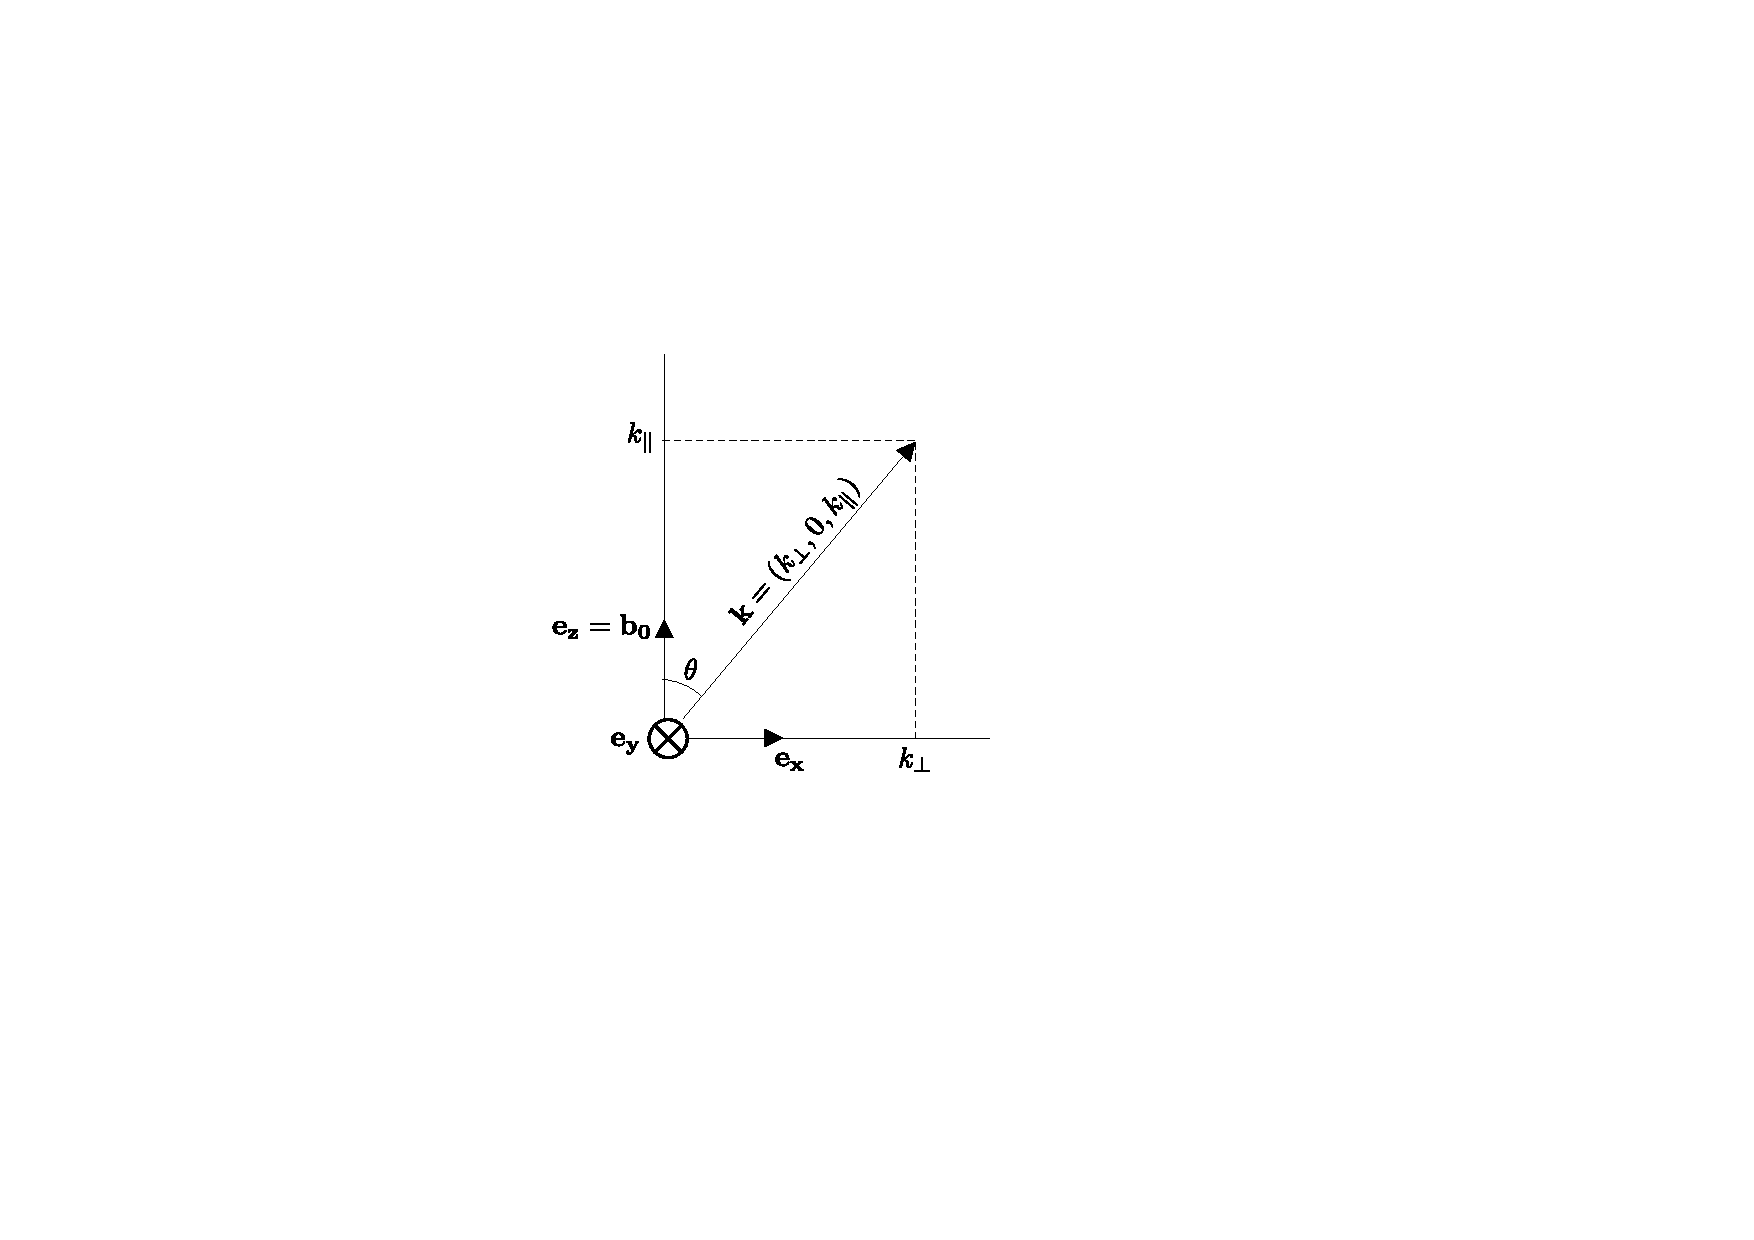
\includegraphics[width=0.6\linewidth,trim=9.3cm 7.8cm 13cm 7cm, clip=true]{./Part_1/images/schema_kplan.pdf}
\caption{Système de coordonnées et vecteur d'onde dans le cadre linéaire.}
\label{fig:schema_kplan}
\end{wrapfigure}

La deuxième étape consiste à passer dans l'espace de Fourier, c'est-à-dire remplacer $\partial_t$ par la pulsation $-i\omega$ et $\nabla$ par le vecteur d'onde $i\boldsymbol{k}$. On supposera sans perte de généralité, le système de coordonnées cartésiennes orienté tel que $\boldsymbol{e_z} = \boldsymbol{b_0}$ et la composante suivant $\boldsymbol{e_y}$ du vecteur d'onde, $k_y = 0$. On notera $k$ la norme du vecteur d'onde, $k_{\parallel}$ sa composante le long de $\boldsymbol{e_z}$, parallèle au champ magnétique moyen, $k_{\perp}$ sa composante le long de $\boldsymbol{e_x}$ et $\theta$ l'angle formé avec $\boldsymbol{e_z}$ (voir \figref{fig:schema_kplan}).
Le système \acs{IMHD} devient alors : 
\begin{eqnarray}
 \label{eq:lin_inc_v} \omega \boldsymbol{v_{1}}  + v_{A0} k_{\parallel} \boldsymbol{v_{A1}} - \frac{1}{\rho_0}  p_{*1} \boldsymbol{k}&=& 0 ,\\
 \label{eq:lin_inc_b} \omega \boldsymbol{v_{A1}}  +  v_{A0} k_{\parallel}  \boldsymbol{v_{1}}&=& 0 ,\\
 \label{eq:lin_inc_r} \boldsymbol{k} \cdot \boldsymbol{v_{1}} = 0 \qquad \boldsymbol{k} \cdot \boldsymbol{v_{A1}}  &=& 0 .
\end{eqnarray}

Ensuite, on injecte les équations \eqref{eq:lin_inc_b} et \eqref{eq:lin_inc_r} dans l'équation \eqref{eq:lin_inc_v} : 
\begin{itemize}
    \item $\boldsymbol{k} \cdot \eqref{eq:lin_inc_v} \Rightarrow  p_{*1} =0$, en excluant le cas trivial où $\boldsymbol{k}=0$. La pression totale n'est donc bien reliée qu'aux non-linéarités du système.
    \item $\omega \cdot \eqref{eq:lin_inc_v} \Rightarrow (\omega^2   - (\boldsymbol{k} \cdot \boldsymbol{v_{A0}})^2 ) \boldsymbol{v_{1}} = 0$ (dite équation de dispersion), d'où la relation de dispersion :  
    \begin{equation}
        \label{eq:lin_inc_disp} \omega = \pm \boldsymbol{k} \cdot \boldsymbol{v_{A0}} = \pm v_{A0} k_{\parallel} =  \pm v_{A0} k \cos \theta .
    \end{equation}
    \item \eqref{eq:lin_inc_b} et \eqref{eq:lin_inc_disp} $ \Rightarrow \boldsymbol{v_{1}} = \pm \boldsymbol{v_{A1}}$.
    \item $ p_{*1} =0 \Rightarrow p_{1} = - v_{A0} v_{A1z}$ .
\end{itemize}
La relation de dispersion \eqref{eq:lin_inc_disp} nous indique qu'il peut y avoir dans le système \acs{IMHD}, des ondes dites d'Alfvén, couplant champ magnétique et champ de vitesse. 
Généralement, pour obtenir la polarisation d'une onde, on injecte sa relation de dispersion dans le système. Dans le cas du système \acs{IMHD}, le système s'annule alors complètement. La polarisation de l'onde d'Alfvén dans le cas \acs{IMHD}, est définie par $\boldsymbol{k} \cdot \boldsymbol{v_{A1}}  = 0 $ qui indique que $\boldsymbol{v_{A1}} $ doit être perpendiculaire à $\boldsymbol{k}$. Or $\boldsymbol{k}$ est dans le plan $\boldsymbol{e_x}-\boldsymbol{e_z}$. Donc $\boldsymbol{v_{A1}} $ est polarisé suivant une combinaison linéaire des vecteurs $\boldsymbol{e_y}$ et $(-\cos \theta, 0, \sin \theta)$. Le mode d'Alfvén est donc dégénéré, il est formé d'un mode dit incompressible, polarisé suivant $\boldsymbol{e_y}$, et d'un mode dit pseudo-alfvénique, polarisé suivant $(-\cos \theta, 0, \sin \theta)$.

L'onde d'Alfvén est très importante en physique des plasmas, elle est, en effet, solution exacte du système \acs{IMHD} linéaire et non linéaire. En turbulence, elle peut donc alimenter la cascade. Lorsque la cascade est développée par des ondes, on parlera de turbulence d'onde. De plus, deux régimes existent :  la turbulence faible où la cascade d'énergie est supposément développée par des interactions faiblement non-linéaires entre paquets d'ondes et, la turbulence forte où ondes et structures cohérentes (de type vortex par exemple) coexistent et entretiennent la cascade. 

\section{Décrire la cascade turbulente incompressible avec une loi exacte}
\label{sec-113}
La théorie des lois exactes, nommée ainsi car aucune hypothèse de linéarisation ou perturbative n'est supposée pour les obtenir, s'appuie sur les hypothèses de Kolmogorov exposées et illustrées dans le Chapitre \ref{ch-01} (voir synthèse \ref{synt-01}) et rappelées ci-après. On se réfèrera au chapitre \ref{ch-01} à propos des notations. Historiquement, de multiples versions de la loi exacte décrivant la cascade \acs{IMHD} et de la méthode pour l'obtenir existent [\cite{politano_von_1998,galtier_origin_2018,macbride_turbulent_2008}]. On la nommera dans la suite \acs{PP98} du nom des deux chercheuses ayant dérivé la première version en 1998.

D'après les hypothèses de Kolmogorov, la zone inertielle est définie comme l'ensemble des échelles où le tranfert s'effectue conservativement. L'énergie totale (cinétique + magnétique) étant un invariant du système \acs{IMHD}, elle peut a priori cascader de manière conservative. 
Une cascade d'énergie implique une source d'injection et un canal de dissipation, respectivement aux grandes et petites échelles. Le canal de dissipation transfert l'énergie des champs électromagnétiques vers les particules du plasma. Cette énergie sera visible dans la fonction de distribution des particules à travers une augmentation de sa largeur (chauffage) ou un décalage de la moyenne (accélération). Dans le cadre \acs{IMHD}, les dissipations généralement admises sont des dissipations visqueuses ou résistives qui s'accompagnent d'une variation d'entropie. 
Le canal d'injection est nécessaire pour entretenir la cascade et compenser la dissipation dans le bilan énergétique (dans le cas incompressible) [\cite{galtier_physique_2021}]. Pour refléter cela dans les équations, on va ajouter une force $\boldsymbol{f_c}$ d'injection agissant à grande échelle et un terme dissipatif (visqueux), $\boldsymbol{d_c}$, agissant à petite échelle, dans l'équation \eqref{eq:model_inc_v} et, pour permettre la visualisation de ce que deviennent ces sources si elles sont définies magnétiquement, on va ajouter $\boldsymbol{f_m}$ et $\boldsymbol{d_m}$ (résistif) dans l'équation d'induction \eqref{eq:model_inc_b}. On restera dans un cadre général en ne détaillant pas leur contenu. Ainsi :
\begin{eqnarray}
\label{eq:turb_inc_v} \partial_t \boldsymbol{v} + \boldsymbol{v} \cdot \nabla \boldsymbol{v} -  \boldsymbol{v_A} \cdot \nabla \boldsymbol{v_A} + \frac{1}{\rho_0} \nabla p_* &=&  \boldsymbol{f_c} + \boldsymbol{d_c} , \\
\label{eq:turb_inc_b}  \partial_t \boldsymbol{v_A} + \boldsymbol{v} \cdot \nabla \boldsymbol{v_A} -  \boldsymbol{v_A} \cdot \nabla \boldsymbol{v}&=& \boldsymbol{f_m} + \boldsymbol{d_m} ,\\
\label{eq:turb_inc_r}  \nabla \cdot \boldsymbol{v} = 0, && \nabla \cdot \boldsymbol{v_A} = 0.
\end{eqnarray}

Maintenant, si l'on veut une loi exacte sur l'énergie totale, on doit choisir une fonction de corrélation qui, lorsque $\boldsymbol{x'}= \boldsymbol{x}$, est égale à l'énergie totale moyenne, ici $\left<E_{tot}\right> = \left<E_c + E_m\right> = \left<\frac{1}{2} \rho_0 \boldsymbol{v}^2 + \frac{1}{2} \rho_0 \boldsymbol{v_A}^2\right>$. Cela nous donne bien des choix de formulation : 
\[\left<\sqrt{E_{tot}} \cdot \sqrt{E'_{tot}}\right>, \qquad \left<\sqrt{E_c} \cdot \sqrt{E'_c} + \sqrt{E_m} \cdot \sqrt{E'_m} \right>,\] et pourquoi pas d'autres puissances ? Ici, c'est la même quantité à une constante près, mais on pourrait avoir à choisir en $\boldsymbol{B}$ ou $\boldsymbol{v_A}$, ou encore utiliser les variables d'Elsässer. Une autre possibilité est de définir cette fonction à l'aide des incréments de quantités (voir par exemple \cite{antonia_analogy_1997}). Avec une telle fonction, on obtient naturellement son annulation lorsque $\boldsymbol{x'}= \boldsymbol{x}$. Du choix de la fonction de corrélation va dépendre la difficulté du calcul, la sauvegarde du sens physique (que voudrait dire $\boldsymbol{v}^{1/5}$ ?) et potentiellement l'élégance et la compacité du résultat. Une question fondamentale subsiste et ne sera qu'en partie traitée dans cette thèse : regarde-t-on la même chose quel que soit le choix de fonction de corrélation ?\footnote{On regardera la différence analytique entre les fonctions de type incrémentale ou non (traitée numériquement dans les cadres \ac{MHDH} incompressible et compressible par [\cite{ferrand_exact_2019,ferrand_-depth_2022}]). La question de la convergence des taux de cascade obtenus avec des lois du même type (incrémental ou non) mais différentes formulations (exemple des différentes puissances) reste un problème ouvert qui n'a, à notre connaissance, pas été traité rigoureusement.} On prendra comme exemple la fonction d'auto-corrélation pour chaque canal d'énergie : $\mathcal{R} = \frac{1}{2} \rho_0\left< \boldsymbol{v} \cdot \boldsymbol{v'} + \boldsymbol{v_A} \cdot \boldsymbol{v'_A}\right>$, $\rho_0/2$ étant une constante dans ce cadre incompressible. 

Ensuite, on doit dériver une équation pour cette fonction de corrélation, elle s'obtient en notant que $\partial_t \mathcal{R} = \frac{1}{2} \rho_0 (\left<\partial_t(\boldsymbol{v}) \cdot \boldsymbol{v'} + \boldsymbol{v} \cdot \partial_t(\boldsymbol{v'}) \right> + \left<\partial_t(\boldsymbol{v_A}) \cdot \boldsymbol{v'_A} + \boldsymbol{v_A} \cdot \partial_t(\boldsymbol{v'_A}) \right>)$ et en remplaçant les dérivées temporelles grâce aux équations \eqref{eq:turb_inc_v} et \eqref{eq:turb_inc_b}. Pour alléger la démonstration, on peut noter que $\left<\partial_t(\boldsymbol{v'}) \cdot \boldsymbol{v}\right> $ est le conjugué de $\left<\partial_t(\boldsymbol{v}) \cdot \boldsymbol{v'}\right> $, c'est-à-dire en échangeant les rôles (prime ou pas) de chacun des points. Ainsi, on obtient en jouant un peu avec l'hypothèse d'homogénéité statistique et les contraintes \eqref{eq:turb_inc_r} : 
\begin{eqnarray}
\label{eq:turb_inc_v1} \left<\boldsymbol{v'} \cdot \partial_t \boldsymbol{v}\right> &=&  \nabla_{\boldsymbol{\ell}} \cdot \left< \boldsymbol{v'} \cdot \boldsymbol{v}\boldsymbol{v}-\boldsymbol{v'} \cdot \boldsymbol{v_A}   \boldsymbol{v_A}\right> +  \left<\boldsymbol{v'} \cdot \boldsymbol{f_c}+\boldsymbol{v'} \cdot \boldsymbol{d_c}\right> ,\\
\label{eq:turb_inc_b1}\left<\boldsymbol{v'_A} \cdot \partial_t \boldsymbol{v_A}\right> &=& \nabla_{\boldsymbol{\ell}} \cdot \left< \boldsymbol{v'_A} \cdot \boldsymbol{v_A}\boldsymbol{v}-\boldsymbol{v'_A} \cdot \boldsymbol{v}\boldsymbol{v_A}\right>  +  \left<\boldsymbol{v'_A} \cdot \boldsymbol{f_m}+\boldsymbol{v'_A} \cdot \boldsymbol{d_m}\right>,
\end{eqnarray}
puisque $ - \left<\boldsymbol{v'} \cdot \nabla p_*\right> = \nabla_{\boldsymbol{\ell}} \cdot \left< p_* \boldsymbol{v'}\right> = \left<p_* \nabla' \cdot \boldsymbol{v'}\right> = 0$. 

On peut  chercher à faire apparaître par factorisation dans les termes dit <<de flux>> (sous l'opérateur $\nabla_{\boldsymbol{\ell}} $) des équations \eqref{eq:turb_inc_v1} et \eqref{eq:turb_inc_b1}, des fonctions de structure, c'est-à-dire des multiplications d'incréments tel que $\left<\delta \boldsymbol{v} \cdot \delta \boldsymbol{v} \delta \boldsymbol{v} \right>$. Via les hypothèses d'homogénéité et les contraintes \eqref{eq:turb_inc_r}, on peut faire ainsi ressortir : 
\begin{eqnarray}
\label{eq:turb_inc_fs1} \nabla_{\boldsymbol{\ell}} &\cdot& \left<\delta \boldsymbol{v} \cdot \delta \boldsymbol{v} \delta \boldsymbol{v} \right> \nonumber \\
 &=&  \nabla_{\boldsymbol{\ell}} \cdot \left<  \boldsymbol{v'} \cdot \boldsymbol{v'} \boldsymbol{v'} - \boldsymbol{v} \cdot \boldsymbol{v} \boldsymbol{v} - \boldsymbol{v'} \cdot \boldsymbol{v'} \boldsymbol{v} + \boldsymbol{v} \cdot \boldsymbol{v} \boldsymbol{v'} + 2 \boldsymbol{v} \cdot \boldsymbol{v'} \boldsymbol{v} - 2 \boldsymbol{v'} \cdot \boldsymbol{v} \boldsymbol{v'}\right>  \nonumber\\
  &=& 2 \nabla_{\boldsymbol{\ell}} \cdot \left< \boldsymbol{v} \cdot \boldsymbol{v'} \boldsymbol{v} - \boldsymbol{v'} \cdot \boldsymbol{v} \boldsymbol{v'}\right>.
\end{eqnarray}
Et de même : 
\begin{eqnarray}
\label{eq:turb_inc_fs2}  \nabla_{\boldsymbol{\ell}} \cdot \left<\delta \boldsymbol{v_A} \cdot \delta \boldsymbol{v_A} \delta \boldsymbol{v} \right>  &=& 2 \nabla_{\boldsymbol{\ell}} \cdot \left< \boldsymbol{v_A} \cdot \boldsymbol{v'_A} \boldsymbol{v} - \boldsymbol{v'_A} \cdot \boldsymbol{v_A} \boldsymbol{v'}\right> ,\\
\label{eq:turb_inc_fs3}   \nabla_{\boldsymbol{\ell}} \cdot \left<\delta \boldsymbol{v} \cdot \delta \boldsymbol{v_A} \delta \boldsymbol{v_A} \right>  &=&  \nabla_{\boldsymbol{\ell}} \cdot \left< \boldsymbol{v} \cdot \boldsymbol{v'_A} \boldsymbol{v_A} - \boldsymbol{v'} \cdot \boldsymbol{v_A} \boldsymbol{v'_A} + \boldsymbol{v'} \cdot \boldsymbol{v_A} \boldsymbol{v_A} - \boldsymbol{v} \cdot \boldsymbol{v'_A} \boldsymbol{v'_A}\right> .\quad
\end{eqnarray}
Les fonctions de structure d'ordre 3, $\left<\delta \boldsymbol{v} \cdot \delta \boldsymbol{v} \delta \boldsymbol{v} \right>$ et $\left<\delta \boldsymbol{v_A} \cdot \delta \boldsymbol{v_A} \delta \boldsymbol{v} \right>$, rappellent la convection de l'énergie, respectivement cinétique et magnétique, par le champ de vitesse et présente dans l'équation d'énergie totale \eqref{eq:model_inc_e}, et $\left<\delta \boldsymbol{v} \cdot \delta \boldsymbol{v_A} \delta \boldsymbol{v_A} \right>$ rappelle la convection de l'hélicité croisée par le champ magnétique.

Ainsi, l'équation de la fonction de corrélation de l'énergie totale obtenue avec $\mathcal{R} = \left<\frac{1}{2} \rho_0 \boldsymbol{v} \cdot \boldsymbol{v'} + \frac{1}{2} \rho_0 \boldsymbol{v_A} \cdot \boldsymbol{v'_A}\right>$ peut s'écrire :
\begin{eqnarray}
\label{eq:turb_inc_KHM}    \partial_t \mathcal{R} &=& \frac{1}{4} \rho_0 \nabla_{\boldsymbol{\ell}} \cdot \left< \delta \boldsymbol{v} \cdot \delta \boldsymbol{v} \delta \boldsymbol{v} + \delta \boldsymbol{v_A} \cdot \delta \boldsymbol{v_A} \delta \boldsymbol{v} + 2 \delta \boldsymbol{v} \cdot \delta \boldsymbol{v_A} \delta \boldsymbol{v_A}\right> \\
 \label{eq:turb_inc_KHMinj}    &&+ \frac{1}{2} \rho_0  \left<\boldsymbol{v'} \cdot \boldsymbol{f_c} + \boldsymbol{v} \cdot \boldsymbol{f'_c} + \boldsymbol{v'_A} \cdot \boldsymbol{f_m} + \boldsymbol{v_A} \cdot \boldsymbol{f'_m}\right> \\
 \label{eq:turb_inc_KHMdiss}    &&+ \frac{1}{2} \rho_0 \left<\boldsymbol{v'} \cdot \boldsymbol{d_c} +\boldsymbol{v} \cdot \boldsymbol{d'_c} + \boldsymbol{v'_A} \cdot \boldsymbol{d_m} + \boldsymbol{v_A} \cdot \boldsymbol{d'_m}\right>.
\end{eqnarray}
Dans le terme de droite, la première ligne décrit la cascade non-linéaire ($\varepsilon_{NL} = $  \eqref{eq:turb_inc_KHM}), la deuxième, l'injection au taux $\varepsilon_F$ ($=$ \eqref{eq:turb_inc_KHMinj}), et la troisième, la dissipation ($\varepsilon_D =$  \eqref{eq:turb_inc_KHMdiss}). Les contributions magnétiques viennent se mêler aux contributions cinétiques présentes dans chaque taux et vues dans le cadre \ac{HD} (voir Chapitre \ref{ch-01}).  Cette équation du type \acs{KHM} est valable dans et en dehors de la zone inertielle. 

En $\boldsymbol{\ell} = 0$, on retrouve l'équation de densité d'énergie totale moyenne du système : $\partial_t \left<E_{tot}\right> = \left<E_F\right> + \left<E_D\right>$ avec $\left<E_F\right> = \rho_0 \left<\boldsymbol{v} \cdot \boldsymbol{f_c} + \boldsymbol{v_A} \cdot \boldsymbol{f_m} \right>$, la densité d'énergie moyenne injectée et $\left<E_D\right> = \rho_0 \left<\boldsymbol{v} \cdot \boldsymbol{d_c} + \boldsymbol{v_A} \cdot \boldsymbol{d_m}\right>$, la densité d'énergie moyenne dissipée. 
Si le système est conservatif, $\left<E_F\right> = -  \left<E_D\right> $. Afin que $\left<E_F\right> = -  \left<E_D\right>$ soit respecté $\varepsilon_F$ ne doit pas s'annuler aux échelles où le forçage n'a pas d'influence mais plutôt être égal à $\left<E_F\right>$. $\varepsilon_F (\ell)$ ne représente donc pas l'énergie qui est injectée à l'échelle $\ell$ mais plutôt l'énergie qui a été injectée dans la cascade aux échelles $>\ell$, où le forçage est actif.

En appliquant l'hypothèse de séparation d'échelle, on obtient la loi de type K41 donnée par $\varepsilon = - \varepsilon_{NL}$ : 
\begin{eqnarray}
\label{eq:turb_inc_ELK}     \varepsilon &=& - \frac{1}{4} \rho_0 \nabla_{\boldsymbol{\ell}} \cdot \left< \delta \boldsymbol{v} \cdot \delta \boldsymbol{v} \delta \boldsymbol{v} + \delta \boldsymbol{v_A} \cdot \delta \boldsymbol{v_A} \delta \boldsymbol{v} + 2 \delta \boldsymbol{v} \cdot \delta \boldsymbol{v_A} \delta \boldsymbol{v_A}\right> .
\end{eqnarray}
Cette équation est la loi exacte \acs{PP98} pour l'énergie totale du modèle \acs{IMHD}, obtenue à partir de la théorie de Kolmogorov. Ce lien entre le taux de cascade et l'anomalie dissipative $\varepsilon$ (voir synthèse \ref{synt-01}) nous permet, dans le vent solaire par exemple, d'estimer le taux de dissipation permise par la turbulence pour répondre par exemple au problème du chauffage (décrit dans le chapitre \ref{ch-02}, voir aussi [\cite{smith_dependence_2006,sorriso-valvo_observation_2007,stawarz_turbulent_2009,osman_proton_2013}]). 

Phénoménologiquement, $\varepsilon$ étant supposé constant et avec l'hypothèse d'isotropie, on remarque que : $(\delta \boldsymbol{v})^3 \sim (\delta \boldsymbol{v_A})^3 \sim \varepsilon \ell => (\delta \boldsymbol{v})^2 \sim (\delta \boldsymbol{v_A})^2 \sim \ell^{2/3}$, ce qui donne les spectres 1D d'énergie cinétique et magnétique en $E(k) \sim k(\delta \boldsymbol{v}(k))^2  \sim k(\delta \boldsymbol{v_A}(k))^2  \sim k^{-5/3}$. On retrouve ainsi la loi phénoménologique des spectres en $-5/3$ de Kolmogorov étendue aux fluides magnétisés.\footnote{Lorsque le champ magnétique est important, de l'anisotropie apparait dans l'espace de Fourier entre la direction parallèle au champ magnétique et le plan perpendiculaire. La description phénoménologique doit donc être modifiée, par exemple avec la condition dite de "critical balance" [\cite{goldreich_toward_1995,horbury_anisotropic_2008}].}

Pour en revenir à la différence entre les fonctions de corrélation, regardons ce qu'il se passe si l'on considère une fonction incrémentale, par exemple $\mathcal{S} =  \left<\frac{1}{2} \rho_0 \delta \boldsymbol{v}^2 + \frac{1}{2} \rho_0 \delta \boldsymbol{v_A}^2\right>$ formée de fonctions de structure d'ordre 2 qui rappelle celles d'ordre 3 impliquées dans le taux de cascade. On remarque que $\mathcal{S} = 2\left<E_{tot}\right> - 2\mathcal{R}$. Ainsi la loi exacte KHM \eqref{eq:turb_inc_KHM} devient : 
\begin{eqnarray}
\label{eq:turb_inc_KHMs}    \partial_t \mathcal{S} &=& -\frac{1}{2} \rho_0 \nabla_{\boldsymbol{\ell}} \cdot \left< \delta \boldsymbol{v} \cdot \delta \boldsymbol{v} \delta \boldsymbol{v} + \delta \boldsymbol{v_A} \cdot \delta \boldsymbol{v_A} \delta \boldsymbol{v} + 2 \delta \boldsymbol{v} \cdot \delta \boldsymbol{v_A} \delta \boldsymbol{v_A}\right> \\
    &&+ \rho_0 \left<\delta \boldsymbol{v} \cdot \delta \boldsymbol{f_c} + \delta \boldsymbol{v_A} \cdot \delta \boldsymbol{f_m} \right> \\
    &&+ \rho_0 \left<\delta \boldsymbol{v} \cdot \delta \boldsymbol{d_c} + \delta \boldsymbol{v_A} \cdot \delta \boldsymbol{d_m}\right>.
\end{eqnarray}
La partie non-linéaire, le taux de cascade, n'est pas impactée. Mais une question émerge : les définitions des taux de forçage et de dissipations dépendants de $\boldsymbol{f_c}$, $\boldsymbol{f_m}$ et $\boldsymbol{d_c}$, $\boldsymbol{d_m}$ extraites de \eqref{eq:turb_inc_KHM} et celles extraites de \eqref{eq:turb_inc_KHMs} sont-elles équivalentes ? Regarder $\mathcal{S}$ ou $\mathcal{R}$ revient à regarder ou une quantité énergétique incrémentale ou celle restant dans le bilan énergétique total moyen $\left<E_{tot}\right> = \mathcal{S}/2 + \mathcal{R}$. C'est la même chose pour les définitions des taux d'injection et de dissipation. Le choix de la définition, incrémentale ou non, des taux, dépend donc du problème que l'on veut étudier et comme on vient de le voir, il est très facile de passer, analytiquement, d'une définition à une autre.  

\newpage
\section{Synthèse sur l'étude de la cascade dans le cadre \acs{IMHD}}
\label{synt-11}
\fcolorbox{blue}{white}{\begin{minipage}[c]{\linewidth}
\paragraph{Modèle contraint tel que $\rho = \rho_0 \Rightarrow \nabla \cdot \boldsymbol{v} = 0 $ : }
\begin{eqnarray}
\label{eq:synth_inc_v} \partial_t \boldsymbol{v} + \boldsymbol{v} \cdot \nabla \boldsymbol{v} -  \boldsymbol{v_A} \cdot \nabla \boldsymbol{v_A} + \frac{1}{\rho_0} \nabla p_* &=&  \boldsymbol{f_c} + \boldsymbol{d_c}, \\
\label{eq:synth_inc_b}\partial_t \boldsymbol{v_A} + \boldsymbol{v} \cdot \nabla \boldsymbol{v_A} -  \boldsymbol{v_A} \cdot \nabla \boldsymbol{v}&=& \boldsymbol{f_m} + \boldsymbol{d_m}, \\
\label{eq:synth_inc_r} \nabla \cdot \boldsymbol{v} = 0 \quad \nabla \cdot \boldsymbol{v_A} &=& 0
.\end{eqnarray}
\end{minipage}}

\fcolorbox{blue}{white}{\begin{minipage}[c]{\linewidth}
\paragraph{Points méthodologiques de linéarisation (voir \figref{fig:schema_kplan}) : }
\begin{itemize}
    \item Négliger toutes quantités ou termes n'étant pas d'ordre 0 ou 1 
    \item $\boldsymbol{v} \simeq \boldsymbol{v_{1}} $, $\boldsymbol{v_A} \simeq \boldsymbol{v_{A0}} + \boldsymbol{v_{A1}}  $ avec $\boldsymbol{v_{A0}} = v_{A0}  \boldsymbol{e_z}$
    \item Passage dans l'espace de Fourier : $\partial_t \rightarrow -i \omega$ et $\nabla \rightarrow i \boldsymbol{k}$ avec  
    \[\boldsymbol{k} = k_{\perp} \boldsymbol{e_x}+ k_{\parallel} \boldsymbol{e_z} = k(\sin \theta \boldsymbol{e_x}+ \cos \theta \boldsymbol{e_z})\].
\end{itemize}

\paragraph{Relation de dispersion linéaire : }  Existence de modes d'Alfvén pouvant participer à la cascade turbulente
\begin{equation}
  \label{eq:synth_inc_lin} \omega = \pm k_{\parallel} v_{A0} = \pm v_{A0} k \cos \theta .
\end{equation}
\end{minipage}}

\fcolorbox{blue}{white}{\begin{minipage}[c]{\linewidth}
\paragraph{Fonctions de corrélation d'énergie totale et moyennes statistiques :}
\begin{itemize}
    \item $\mathcal{R} = \frac{1}{2} \rho_0 \left<\boldsymbol{v} \cdot \boldsymbol{v'} + \boldsymbol{v_A} \cdot \boldsymbol{v'_A}\right>$,
    \item $\mathcal{S} = \frac{1}{2} \rho_0 \left<(\delta \boldsymbol{v})^2 + (\delta \boldsymbol{v_A})^2\right> = 2\left<E_{tot}\right> - 2\mathcal{R}$,
    \item $\left<E_{tot}\right> =  \mathcal{R}(\boldsymbol{\ell} = 0)$, $\left<E_{F}\right> = \varepsilon_{F}(\boldsymbol{\ell} = 0)$, $\left<E_{D}\right> = \varepsilon_{D}(\boldsymbol{\ell} = 0)$.
\end{itemize}

\paragraph{Équations statistiques (densité d'énergie totale moyenne, lois exactes KHM avec $\mathcal{R}$ et $\mathcal{S}$) :}  
\begin{eqnarray}
\label{eq:synth_inc_E} \partial_t \left<E_{tot}\right> &=& \left<E_{F}\right> + \left<E_{D}\right>, \\
 \label{eq:synth_inc_R}    \partial_t \mathcal{R} = - \varepsilon_{NL} + \varepsilon_{F} + \varepsilon_{D} 
    &=& \frac{1}{4} \rho_0 \nabla_{\boldsymbol{\ell}} \cdot \left< \delta \boldsymbol{v} \cdot \delta \boldsymbol{v} \delta \boldsymbol{v} + \delta \boldsymbol{v_A} \cdot \delta \boldsymbol{v_A} \delta \boldsymbol{v} + 2 \delta \boldsymbol{v} \cdot \delta \boldsymbol{v_A} \delta \boldsymbol{v_A}\right> \nonumber \\
    &&+ \frac{1}{2} \rho_0  \left<\boldsymbol{v'} \cdot \boldsymbol{f_c} + \boldsymbol{v} \cdot \boldsymbol{f'_c} + \boldsymbol{v'_A} \cdot \boldsymbol{f_m} + \boldsymbol{v_A} \cdot \boldsymbol{f'_m}\right> \nonumber\\
    &&+ \frac{1}{2} \rho_0 \left<\boldsymbol{v'} \cdot \boldsymbol{d_c} +\boldsymbol{v} \cdot \boldsymbol{d'_c} + \boldsymbol{v'_A} \cdot \boldsymbol{d_m} + \boldsymbol{v_A} \cdot \boldsymbol{d'_m}\right>, \\
 \label{eq:synth_inc_S}   \partial_t \mathcal{S} = - \mathcal{E}_{NL} + \mathcal{E}_{F} + \mathcal{E}_{D} 
    &=&  -\frac{1}{2} \rho_0 \nabla_{\boldsymbol{\ell}} \cdot \left< \delta \boldsymbol{v} \cdot \delta \boldsymbol{v} \delta \boldsymbol{v} + \delta \boldsymbol{v_A} \cdot \delta \boldsymbol{v_A} \delta \boldsymbol{v} + 2 \delta \boldsymbol{v} \cdot \delta \boldsymbol{v_A} \delta \boldsymbol{v_A}\right> \nonumber\\
    &&+ \rho_0 \left<\delta \boldsymbol{v} \cdot \delta \boldsymbol{f_c} + \delta \boldsymbol{v_A} \cdot \delta \boldsymbol{f_m} \right> \nonumber\\ 
    &&+ \rho_0 \left<\delta \boldsymbol{v} \cdot \delta \boldsymbol{d_c} + \delta \boldsymbol{v_A} \cdot \delta \boldsymbol{d_m}\right>.
\end{eqnarray}

\paragraph{Loi exacte PP98 sur les taux d'énergie (type K41) :} 
\begin{eqnarray}
 \label{eq:synth_inc_EL}   \varepsilon &=& - \frac{1}{4} \rho_0 \nabla_{\boldsymbol{\ell}} \cdot \left< \delta \boldsymbol{v} \cdot \delta \boldsymbol{v} \delta \boldsymbol{v} + \delta \boldsymbol{v_A} \cdot \delta \boldsymbol{v_A} \delta \boldsymbol{v} + 2 \delta \boldsymbol{v} \cdot \delta \boldsymbol{v_A} \delta \boldsymbol{v_A}\right>. 
\end{eqnarray}
\end{minipage}}


 


